\documentclass[aspectratio=169]{beamer}


%%% Style
%%% Gabarit de présentation du DMS
\RequirePackage{graphicx}
\usepackage{colortbl}

\usepackage{tikz}

%%% Couleurs
\definecolor{bleu-udem}{RGB}{0, 107, 182}
\definecolor{gris-udem}{RGB}{102, 102, 102}
\definecolor{rouge}{RGB}{204, 0, 0}
\definecolor{vert}{RGB}{153, 204, 0}

\definecolor{intact-red}{RGB}{192, 0, 0}
\definecolor{intact-blue}{RGB}{24, 168, 166}

\usecolortheme{lily}  % désinstalle les couleurs par défaut
\setbeamercolor*{normal text}{fg=black,bg=white}
\setbeamercolor*{alerted text}{fg=rouge}
\setbeamercolor*{example text}{fg=vert}
\setbeamercolor*{structure}{fg=black}

\setbeamercolor*{block title}{fg=white,bg=gris-udem}
\setbeamercolor*{block title alerted}{fg=white,bg=gris-udem}
\setbeamercolor*{block title example}{fg=white,bg=gris-udem}

\setbeamercolor*{block body}{bg=black!10}
\setbeamercolor*{block body alerted}{bg=black!10}
\setbeamercolor*{block body example}{bg=black!10}

\setbeamercolor{item}{fg=bleu-udem}
\setbeamercolor{background canvas}{bg=gris-udem!5}


%%% Liens
\hypersetup{
  colorlinks=true,
  pdfnewwindow=true,
  linkcolor=gris-udem,
  citecolor=bleu-udem,
  filecolor=bleu-udem,
  urlcolor=bleu-udem
}


%%% Canva
\newlength{\textmarginL}
\newlength{\textmarginR}
\setlength{\textmarginL}{7.5mm}
\setlength{\textmarginR}{3.5mm}
%\setlength{\textmarginL}{0mm}
%\setlength{\textmarginR}{0mm}
\setbeamersize{text margin left=\textmarginL, text margin right=\textmarginR}
\newlength{\titleseparator}
\setlength{\titleseparator}{.71\paperwidth}  % distance entre le côté gauche et la barre horizontale (Page titre)
\newenvironment{changemargin}[2]{%
  \begin{list}{}{%
    \setlength{\topsep}{0pt}%
    \setlength{\leftmargin}{#1}%
    \setlength{\rightmargin}{#2}%
    \setlength{\listparindent}{\parindent}%
    \setlength{\itemindent}{\parindent}%
    \setlength{\parsep}{\parskip}%
  }%
  \item[]}{\end{list}}

%%% Images et logo
\newcommand{\insertslidelogo}{\rule{0pt}{.14\paperheight}} % .14\paperheight = .22\paperwidth
\newcommand{\slidelogo}{
  \renewcommand{\insertslidelogo}{
	
\includegraphics[height=.14\paperheight]{figures/template/titlepage_background}
  }
}
\newcommand{\inserttitlelogo}{\rule{0pt}{.16\paperheight}}  % .16\paperheight = .25\paperwidth
\newcommand{\titlelogo}{
  \renewcommand{\inserttitlelogo}{
	
\includegraphics[height=0.16\paperheight]{figures/template/titlepage_background}
  }
}
\newcommand{\inserttitleimage}{\rule{0pt}{.28\paperheight}}
\newcommand{\titleimage}[1]{
  \renewcommand{\inserttitleimage}{
  \includegraphics[height=.28\paperheight, keepaspectratio=true]{#1}
  }
}

%%% Page titre
\setbeamertemplate{title page}{

\begin{changemargin}{-\textmarginL}{-\textmarginR}
%\begin{tabular}{@{}r!{\color{bleu-udem}\vline}@{}l@{}}
% & \inserttitlelogo\\
%\inserttitleimage & \\
%\rule{0pt}{20pt}
%\parbox{\titleseparator}{\flushright\Large{\inserttitle}} & \\
%\parbox{\titleseparator}{\flushright\small{\insertsubtitle}}  & \\
%\rule{0pt}{24pt}
%\parbox{\titleseparator}{\flushright\insertauthor} & \\
%\parbox{\titleseparator}{\flushright\insertinstitute}  & \\
%\rule{0pt}{18pt}
%\parbox{\titleseparator}{\flushright\small{\insertdate}} & \\
%\end{tabular}
\vspace{-9pt}
\begin{tikzpicture}
	\draw (0, 0) node[inner sep=0] {
\includegraphics[width=\paperwidth, height=1.02\paperheight]{figures/template/titlepage_background}};
	\draw (0, 2) node {\parbox{\titleseparator}{\centering \color{white} \Huge{\inserttitle}}};
	\draw (-2, -0.5) node {\parbox{\titleseparator}{\centering \color{white} \Large{\insertauthor}}};
	\draw (-2, -1.25) node {\parbox{\titleseparator}{\centering \color{white} \insertinstitute}};
	\draw (-2, -2.) node {\parbox{\titleseparator}{\centering \color{white} \insertdate}};

\end{tikzpicture}
\end{changemargin}
}


%%% Entête
\setbeamertemplate{frametitle}{%
\vskip-33pt\parbox[c]{.68\paperwidth}{\large\insertframetitle}\vskip4pt%
}
\setbeamertemplate{headline}{%
\vspace{.14\paperheight}

\hspace{20pt}
\color{intact-blue}\rule{0.075\paperwidth}{0.5pt}
\hspace{-5pt}
\color{black}\rule{0.075\paperwidth}{0.5pt}
\hspace{-5pt}
\color{intact-red}\rule{.075\paperwidth}{.5pt}%
}


%%% Pied de page
\beamertemplatenavigationsymbolsempty
\newcommand{\numsubsectionname}{}
\newcommand{\showsubsection}{
  \renewcommand{\numsubsectionname}{%
	\thesection.\thesubsection \; \insertsubsection
  }
}
\newcommand{\insertfootlinetext}{}
\newcommand{\footlinetext}[1]{
  \renewcommand{\insertfootlinetext}{#1}
}
%\setbeamertemplate{footline}{
%{\hfill\color{bleu-udem}\rule{.98\paperwidth}{0.07pt}}%
%\vskip4pt%
%\color{gris-udem}%
%\rule{0.02\paperwidth}{0pt}%
%\numsubsectionname
%\hfill%
%\mbox{\insertfootlinetext\qquad\qquad\insertframenumber}%
%\rule{\textmarginR}{0pt}%
%\vskip4pt%
%}

\setbeamertemplate{footline}{

\hspace{12pt}

\begin{tikzpicture}
	\node[mark size=7.5pt,color=intact-blue] at (0,0) {\pgfuseplotmark{*}};
	\node[mark size=7.5pt,color=intact-red, opacity=0.9] at (0.25,0) {\pgfuseplotmark{*}};
	\draw (0.25, 0) node {\color{white} \insertframenumber};
\end{tikzpicture}
\vspace{12pt}
}




%%% Extensions utiles pour le français
%\usepackage[french]{babel}
%\usepackage[utf8]{inputenc}
%\usepackage[T1]{fontenc}

\usepackage{xcolor}

%%% Extensions utiles pour les math
\usepackage{amsmath}
\usepackage{amsfonts}
\usepackage{bbold}
\usepackage{mathtools}

\DeclareMathOperator*{\argmin}{arg\,min}

%%% Extensions pour les figures
\usepackage{graphicx}
%\usepackage{subfig}
\usepackage{tikz}

%%% for python scripts
\usepackage{listings}
\usepackage{verbatim}

%%% Bibliographie
\usepackage{bibentry}

%%% Informations sur la présentation
\author{Patrice B\'echard}
\institute[Intact]{
\small{Intact Data Lab} \\
\textit{patrice.bechard@intact.net}
}
\title{The Transformer Architecture and Generative Pre-training}
\date{\today}


%%% Préférences (Propre au thème du DMS)
\slidelogo
\titlelogo
%\titleimage{figures/deep_learning_v2.png}  % Image à afficher sur la page titre
\footlinetext{  % À utiliser surtout pour les congrès
\insertshorttitle\quad\insertshortdate\quad\insertshortinstitute
}


\def\signed #1{{\leavevmode\unskip\nobreak\hfil\penalty50\hskip2em
  \hbox{}\nobreak\hfil(#1)%
  \parfillskip=0pt \finalhyphendemerits=0 \endgraf}}

\newsavebox\mybox
\newenvironment{aquote}[1]
  {\savebox\mybox{#1}\begin{quote}}
  {\signed{\usebox\mybox}\end{quote}}

 \usepackage{ragged2e}


%%% Début
\begin{document}

% Title page

\begin{frame}[plain, t]
  \titlepage
\end{frame}

%%%%%%%%%%%%%%%%%%%%%%%%%%%%%%%%%%%%%%%%%%%%%%%%%%%%%%%%%%%%%%%%%%%%%%%%%%%%%%%%%%%%%%%%
% Motivations
%%%%%%%%%%%%%%%%%%%%%%%%%%%%%%%%%%%%%%%%%%%%%%%%%%%%%%%%%%%%%%%%%%%%%%%%%%%%%%%%%%%%%%%%

\begin{frame}{Overview}

\centering {\Large Why are these recent advances important?}
\vspace{.5cm}

\begin{itemize}
	\item \textit{Classical} Neural Machine Translation (NMT) approaches are difficult to parallelize and take a long time to train.
	\item Annotated datasets are expensive to build (time and resources).
	\item We have an \textit{infinite} amount of raw textual data that we can now leverage.
\end{itemize}

\end{frame}

%%%%%%%%%%%%%%%%%%%%%%%%%%%%%%%%%%%%%%%%%%%%%%%%%%%%%%%%%%%%%%%%%%%%%%%%%%%%%%%%%%%%%%%%
% Table of contents
%%%%%%%%%%%%%%%%%%%%%%%%%%%%%%%%%%%%%%%%%%%%%%%%%%%%%%%%%%%%%%%%%%%%%%%%%%%%%%%%%%%%%%%%

\begin{frame}{Plan}
  \tableofcontents
\end{frame}

%%%%%%%%%%%%%%%%%%%%%%%%%%%%%%%%%%%%%%%%%%%%%%%%%%%%%%%%%%%%%%%%%%%%%%%%%%%%%%%%%%%%%%%%
% Neural Machine Translation
%%%%%%%%%%%%%%%%%%%%%%%%%%%%%%%%%%%%%%%%%%%%%%%%%%%%%%%%%%%%%%%%%%%%%%%%%%%%%%%%%%%%%%%%
\section{Neural Machine Translation}

\begin{frame}{Neural Machine Translation}
\centering
\textbf{The Task}
\vspace{1cm}

\raggedright
Translating a source sentence 

$$
\mathbf{X} = \{ \mathbf{x}^{(1)}, \mathbf{x}^{(2)}, \dots, \mathbf{x}^{(n)}\}
$$

into a target sentence 

$$
\mathbf{Y} = \{ \mathbf{y}^{(1)}, \mathbf{y}^{(2)}, \dots, \mathbf{y}^{(m)} \}
$$

\begin{itemize}
	\item In practice, we have huge amounts of parallel texts (e.g. parliament documents from EU, Canada, ...)
\end{itemize}

\end{frame}

\begin{frame}{Neural Machine Translation}
The Sequence to Sequence (Seq2Seq) model \cite{cho2014learning, sutskever2014sequence}

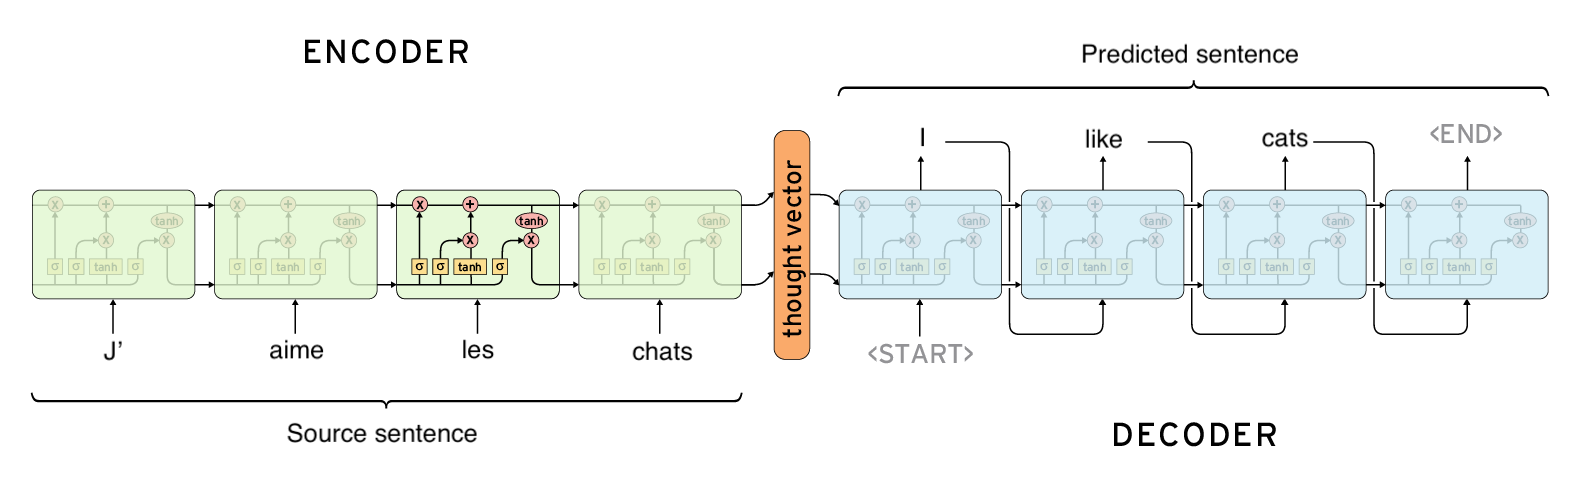
\includegraphics[width=\textwidth]{figures/seq2seq}

\begin{itemize}
	\item Difficult to learn long-term dependencies, even with a LSTM network.
\end{itemize}

\end{frame}

\begin{frame}{Neural Machine Translation}

For a sequence to sequence model (Seq2Seq), we can express the conditional probability of $\mathbf{Y}$ being outputted by the decoder given $\mathbf{X}$ :

$$
p(\mathbf{X}|\mathbf{Y}) = \prod _{t'=1}^{m} p(\mathbf{y}^{(t')}|\mathbf{X}, \mathbf{y}^{(1)}, \dots, \mathbf{y}^{(t'-1)})
$$

Our goal is to maximize the probability of our model producing an accurate translation. Given the \textit{ground truth} translation $\mathbf{Y}$, the source sequence $\mathbf{X}$ and a training set $\mathcal{D}$, we train oure model to maximize the following objective :

$$
\mathcal{L} = \frac{1}{|\mathcal{D}|} \sum _{(\mathbf{X}, \mathbf{Y}) \in \mathcal{D})} \log p(\mathbf{Y}|\mathbf{X})
$$

\end{frame}

\begin{frame}{Neural Machine Translation}
\begin{columns}
\begin{column}{0.5\textwidth}
   \centering
   The Attention Mechanism \cite{bahdanau2014neural, luong2015effective}
   
   \vspace{.5cm}
   \raggedright
   \begin{itemize}
   	\item Shortcut between word from source sentence and target sentence
	\vspace{.5cm}
	\item Allows the model to jointly learn to :
	\begin{itemize}
		\item \textbf{align} words from the source sentence with words from the target sentence;
		\item \textbf{translate} the source sentence to the target sentence.
	\end{itemize}
   \end{itemize}
\end{column}
\begin{column}{0.5\textwidth}  %%<--- here
    \begin{center}
    \vspace{-1.9cm}
    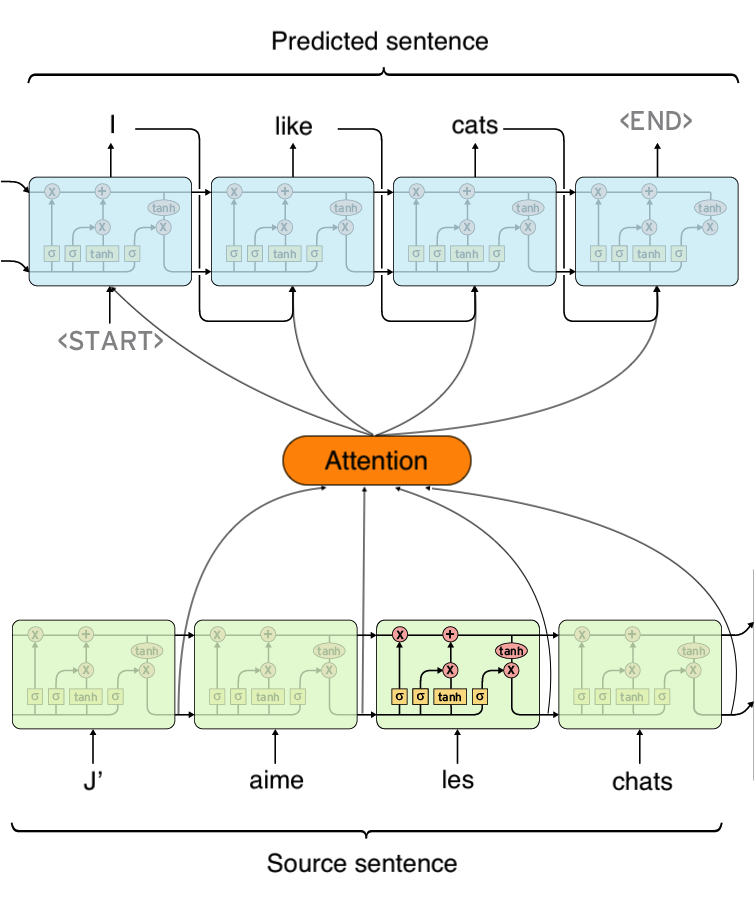
\includegraphics[height=\paperheight]{figures/seq2seq_attn}
    \end{center}
\end{column}
\end{columns}
\end{frame}

\begin{frame}{Neural Machine Translation}
\centering
How to compute attention weights?

\raggedright
\begin{itemize}
	\item We compute a weighted sum of all the encoder's outputs (the \textit{context vector} $\mathbf{c}^{(t')}$) for each predicted word.
\end{itemize}
\vspace{.5cm}
$$
e^{(t', t)} = \mathbf{v}_a ^T \mathrm{tanh} \left( \mathbf{W}_a \mathbf{s}^{(t'-1)} + \mathbf{U}_a \mathbf{h}^{(t)} \right)
$$

$$
\alpha^{(t', t)} = \frac{\exp e^{(t', t)}}{\sum_{t=1}^{n} \exp e^{(t', t)}}
$$

$$
\mathbf{c}^{(t')} = \sum_{t=1} ^{n} \alpha^{(t', t)} \mathbf{h}^{(t)}
$$

\end{frame}

\begin{frame}{Neural Machine Translation}
\begin{columns}
\begin{column}{0.5\textwidth}
   \centering
   Visualizing Attention Weights   
   \vspace{.5cm}
   
   \raggedright
   \begin{itemize}
   	\item Here we visualize the $\alpha^{(t', t)}$ from the previous slide.
   	\item The model learns to align word groups together properly.
   \end{itemize}
\end{column}
\begin{column}{0.5\textwidth}  %%<--- here
    \begin{center}
    \vspace{-1cm}
    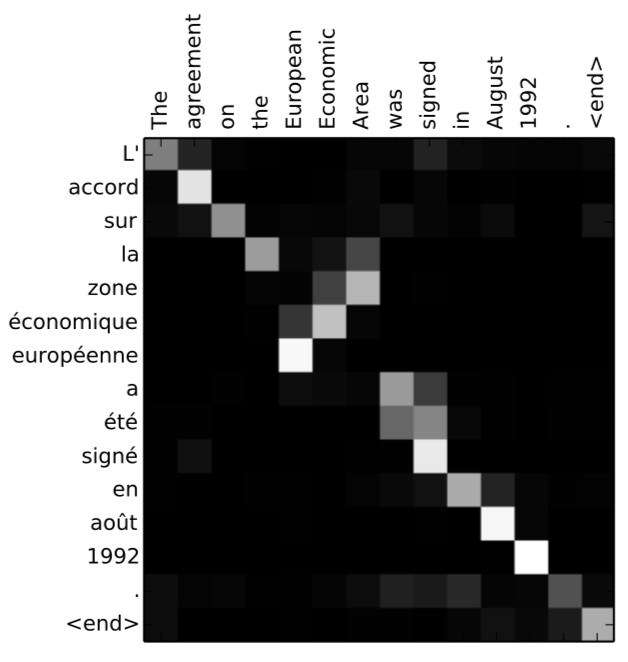
\includegraphics[width=\textwidth]{figures/attention_visualisation}
    \end{center}
\end{column}
\end{columns}
\end{frame}

\begin{frame}{Neural Machine Translation}
\centering Limitations
\vspace{.5cm}

\raggedright
\begin{itemize}
	\item The model is inherently sequential. The computing time depends on the length of the input sequence as well as the output sequence.
	\item In most cases, we know the entirety of the input sequence before beginning the translation. We can try to leverage this in order to process the sequences faster.
	\item Many people have tried to tackle this problem \cite{gehring2017convolutional, kalchbrenner2016neural, gehring2016convolutional}
\end{itemize}
\end{frame}

%%%%%%%%%%%%%%%%%%%%%%%%%%%%%%%%%%%%%%%%%%%%%%%%%%%%%%%%%%%%%%%%%%%%%%%%%%%%%%%%%%%%%%%%
% The Transformer Architecture
%%%%%%%%%%%%%%%%%%%%%%%%%%%%%%%%%%%%%%%%%%%%%%%%%%%%%%%%%%%%%%%%%%%%%%%%%%%%%%%%%%%%%%%%
\section{The Transformer Architecture}

\begin{frame}{The Transformer Architecture}
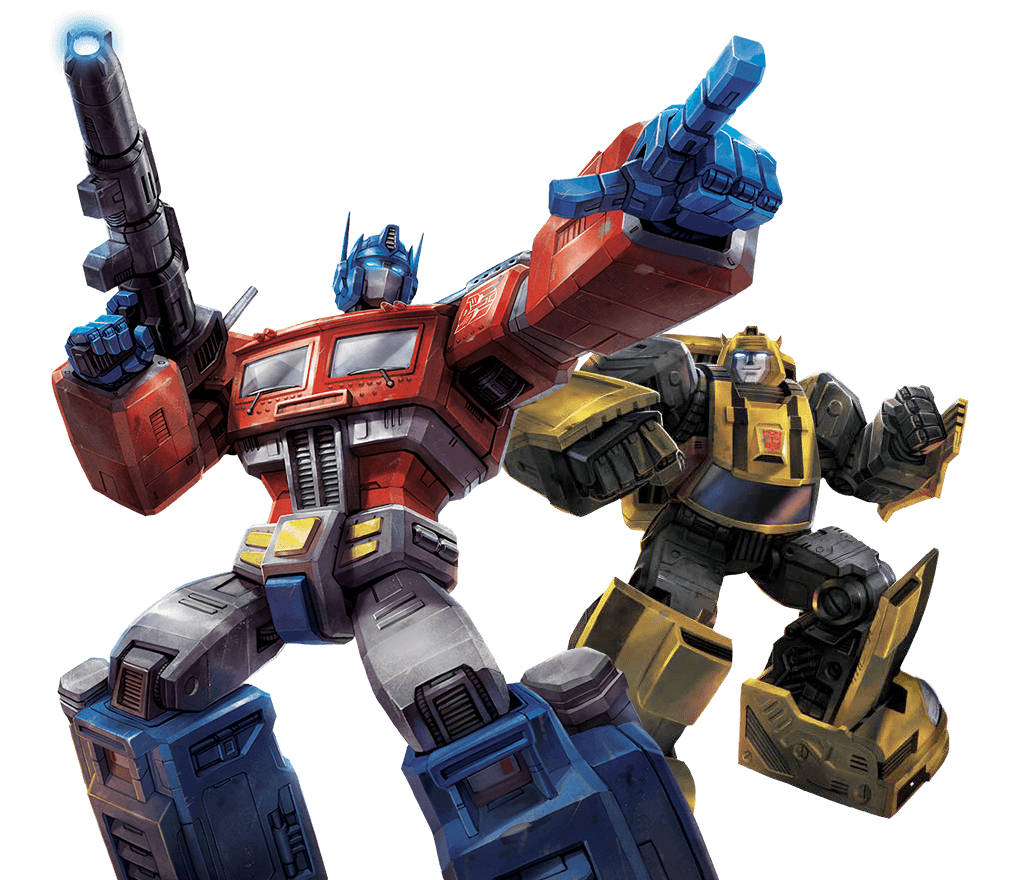
\includegraphics[width=\textwidth]{figures/optimus_prime_bumblebee}
\end{frame}

\begin{frame}{The Transformer Architecture}
\begin{columns}
\begin{column}{0.5\textwidth}
   \centering The Transformer Architecture \cite{vaswani2017attention}
   \vspace{.5cm}
   
   \raggedright
   \begin{itemize}
   	\item No use of recurrent neural networks
	\item We still have the encoder-decoder architecture
	\item Composed of multiple parts :
	\begin{itemize}
		\item Input Embedding
		\item Position Embedding
		\item Multi-Head Attention
		\item Feed Forward Network
	\end{itemize}
   \end{itemize}
\end{column}
\begin{column}{0.5\textwidth}  %%<--- here
    \begin{center}
    \vspace{-1.3cm}
    \begin{figure}
    \begin{overprint}
    	\onslide <1> 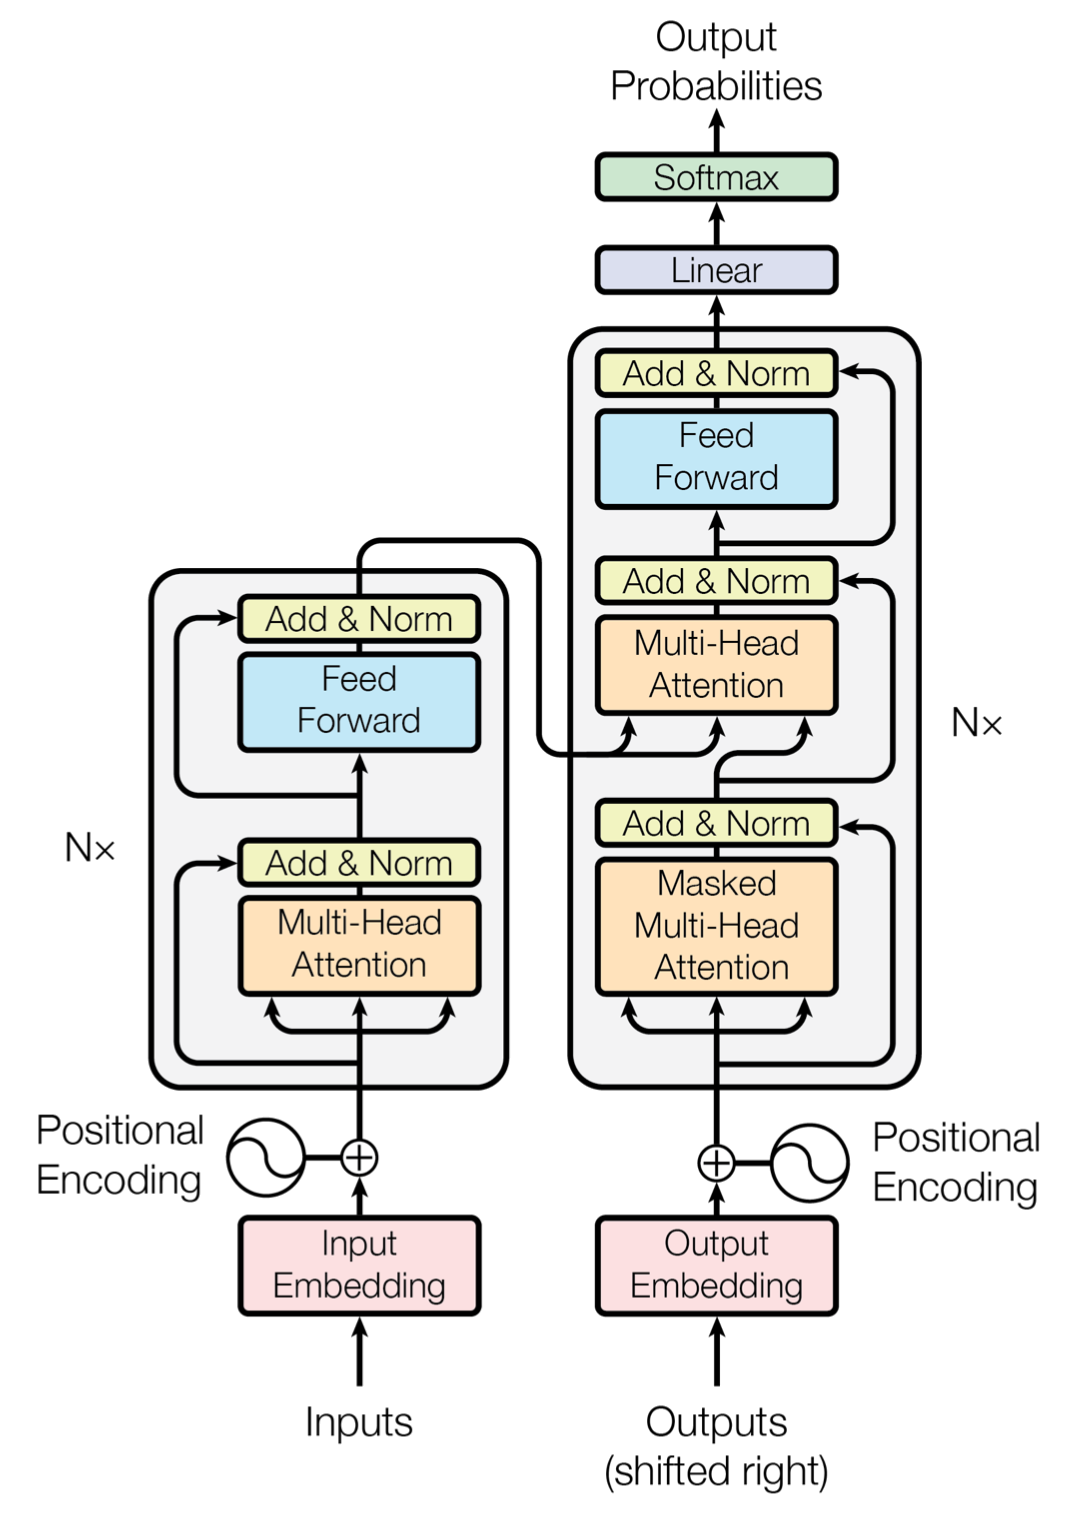
\includegraphics[height=\paperheight]{figures/transformer}
	\onslide <2> 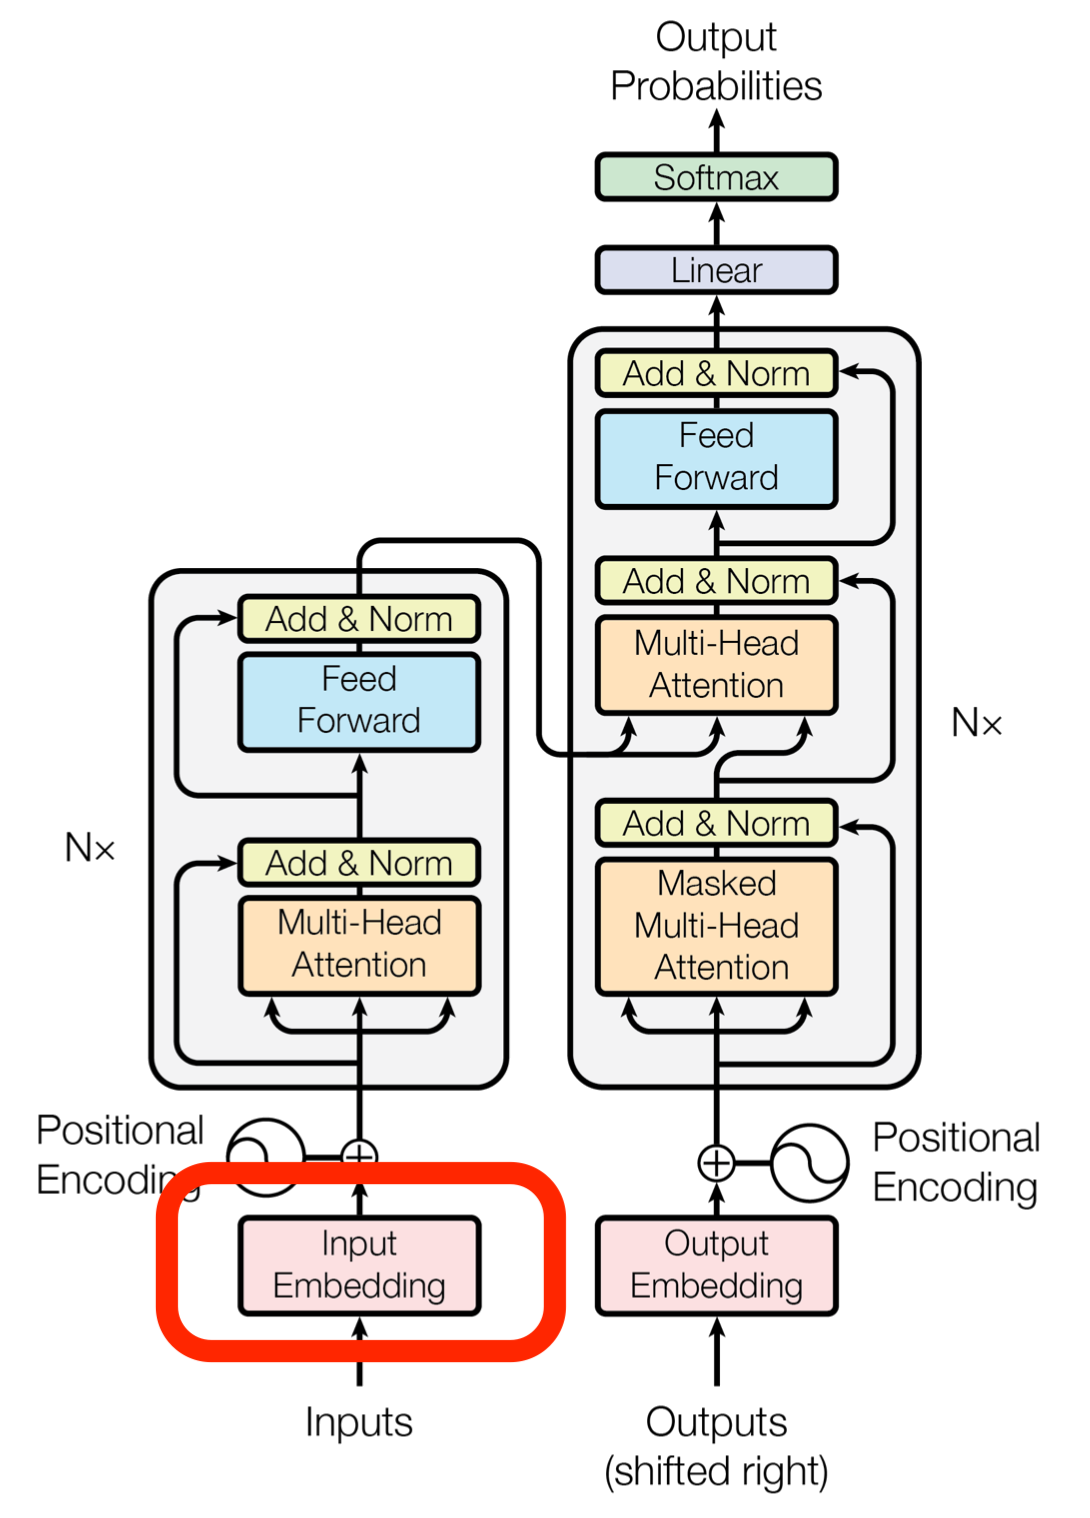
\includegraphics[height=\paperheight]{figures/transformer_in_embed}
	\onslide <3> 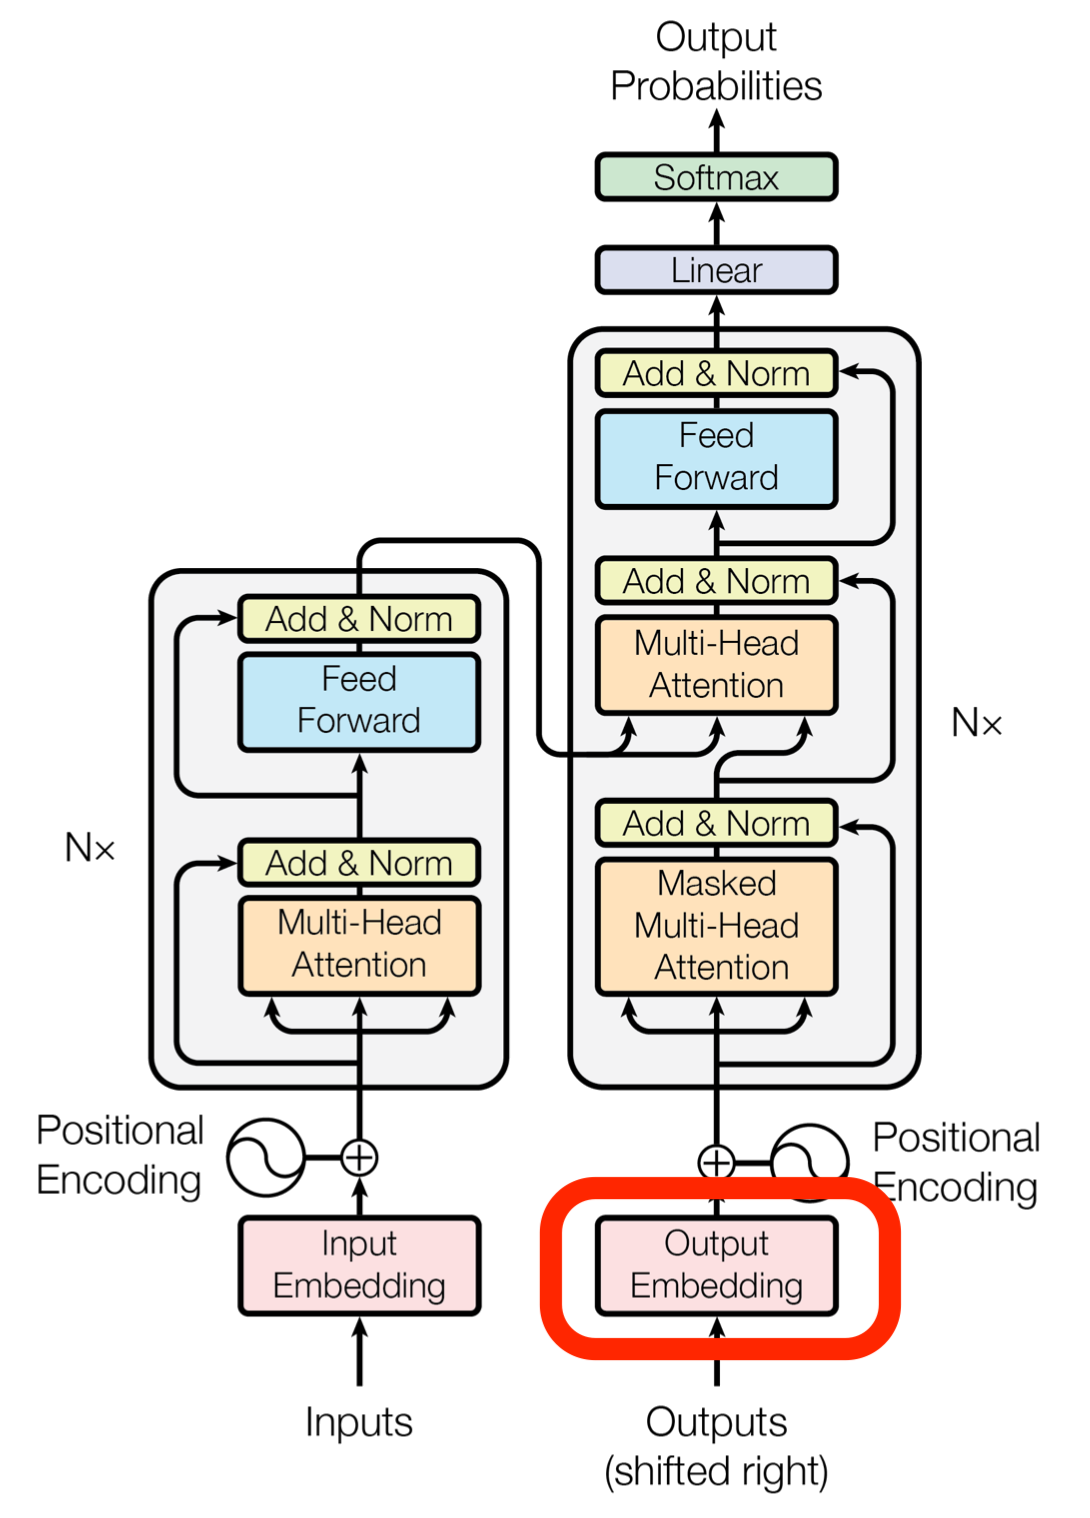
\includegraphics[height=\paperheight]{figures/transformer_out_embed}
    \end{overprint}
    \end{figure}
    \end{center}
\end{column}
\end{columns}
\end{frame}

%%%%%%%%%%%%%%%%%%%%%%%%%%%%%%%%%%%%%%%%%%%%%%%%%%%%%%%%%%%%%%%%%%%%%%%%%%%%%%%%%%%%%%%%
% Transformer (Position Encoding)
%%%%%%%%%%%%%%%%%%%%%%%%%%%%%%%%%%%%%%%%%%%%%%%%%%%%%%%%%%%%%%%%%%%%%%%%%%%%%%%%%%%%%%%%

\begin{frame}{The Transformer Architecture}
\begin{columns}
\begin{column}{0.5\textwidth}
	\centering

   The Transformer Architecture \cite{vaswani2017attention}
   
   	\vspace{.5cm}
	\raggedright
   \begin{itemize}
   	\item No use of recurrent neural networks
	\item We still have the encoder-decoder architecture
	\item Composed of multiple parts :
	\begin{itemize}
		\item Input Embedding
		\item Position Embedding
		\item Multi-Head Attention
		\item Feed Forward Network
	\end{itemize}
   \end{itemize}
\end{column}
\begin{column}{0.5\textwidth}  %%<--- here
    \begin{center}
    \vspace{-1.3cm}
    \begin{figure}
    \begin{overprint}
    	\onslide <1> 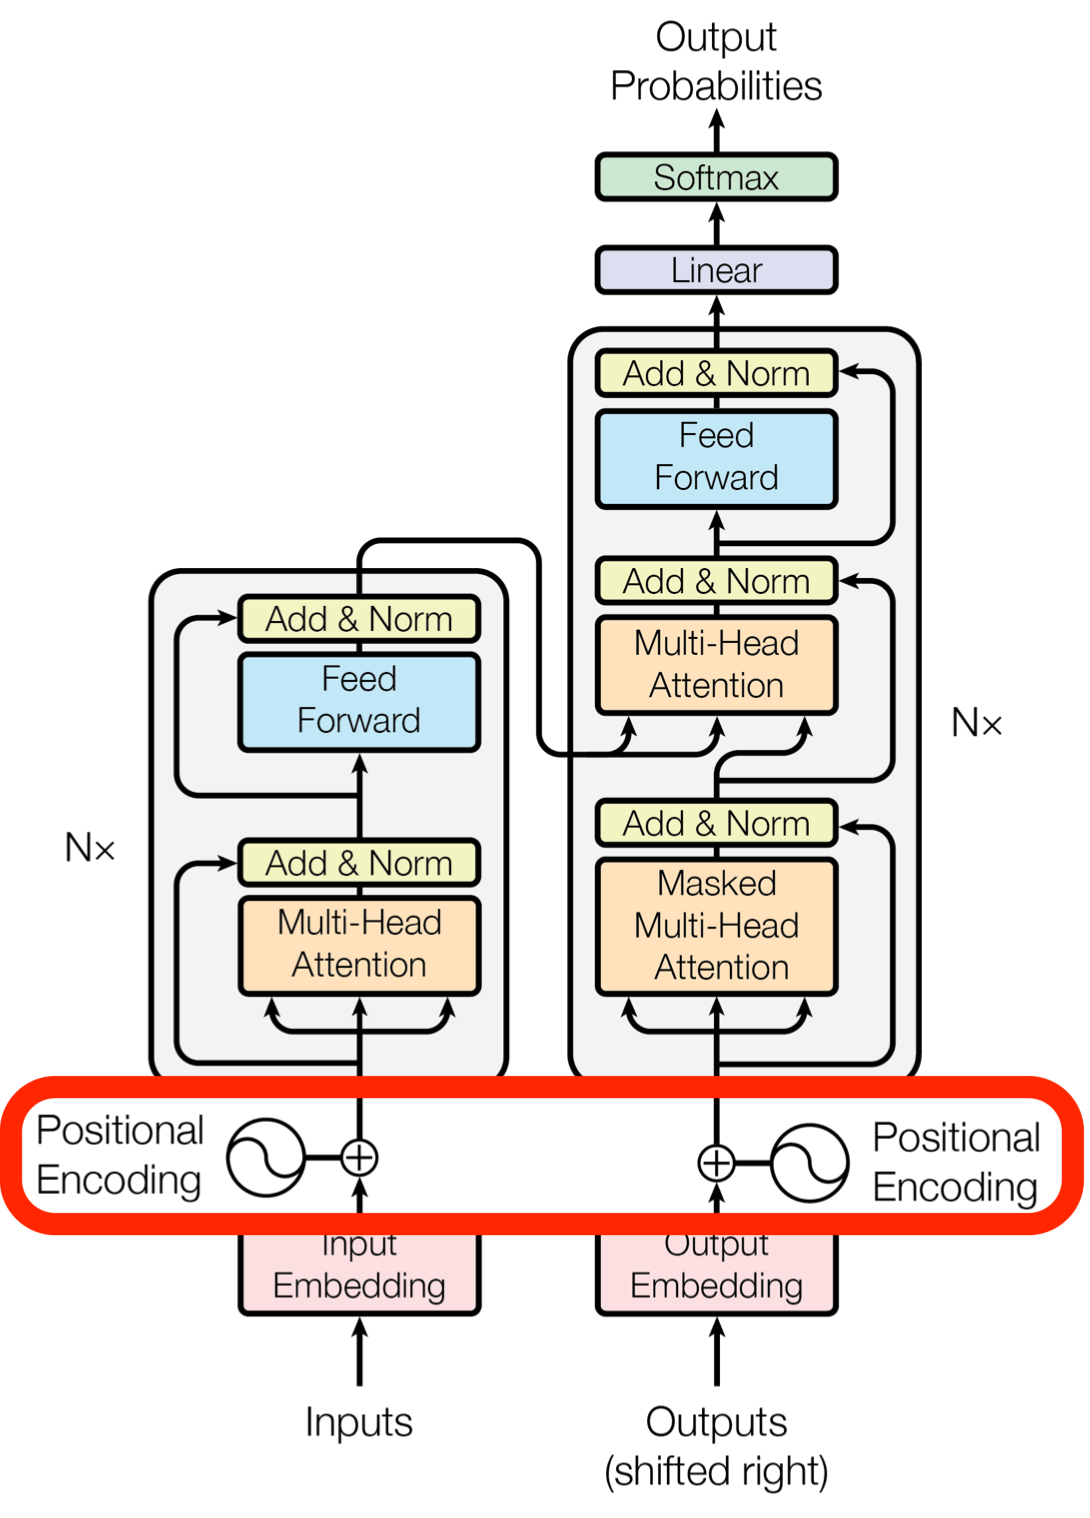
\includegraphics[height=\paperheight]{figures/transformer_pos_embed}
    \end{overprint}
    \end{figure}
    \end{center}
\end{column}
\end{columns}
\end{frame}

\begin{frame}{The Transformer Architecture}

\centering
Position Embeddings
\vspace{.2cm}

\raggedright
\begin{itemize}
	\item Can be either learned (via backpropagation) or defined as a bunch of sines and cosines.
\end{itemize}
\vspace{.2cm}

$$
PE_{(pos, 2i)} = \sin \left(\frac{pos}{10000^{2i/d_{model}}} \right) \qquad PE_{(pos, 2i+1)} = \cos \left(\frac{pos}{10000^{2i/d_{model}}} \right)
$$
\vspace{.3cm}
\centering
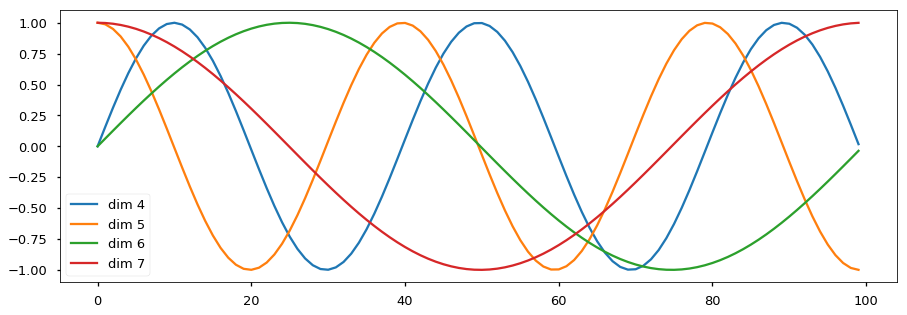
\includegraphics[width=0.7\textwidth]{figures/pos_encoding_sines}

\end{frame}

%%%%%%%%%%%%%%%%%%%%%%%%%%%%%%%%%%%%%%%%%%%%%%%%%%%%%%%%%%%%%%%%%%%%%%%%%%%%%%%%%%%%%%%%
% Transformer Self-Attention
%%%%%%%%%%%%%%%%%%%%%%%%%%%%%%%%%%%%%%%%%%%%%%%%%%%%%%%%%%%%%%%%%%%%%%%%%%%%%%%%%%%%%%%%

\begin{frame}{The Transformer Architecture}
\begin{columns}
\begin{column}{0.5\textwidth}
\centering

   The Transformer Architecture \cite{vaswani2017attention}
 \vspace{.5cm}
 
 \raggedright
   \begin{itemize}
   	\item No use of recurrent neural networks
	\item We still have the encoder-decoder architecture
	\item Composed of multiple parts :
	\begin{itemize}
		\item Input Embedding
		\item Position Embedding
		\item Multi-Head Attention
		\item Feed Forward Network
	\end{itemize}
   \end{itemize}
\end{column}
\begin{column}{0.5\textwidth}  %%<--- here
    \begin{center}
    \vspace{-1.3cm}
    \begin{figure}
    \begin{overprint}
    	\onslide <1> 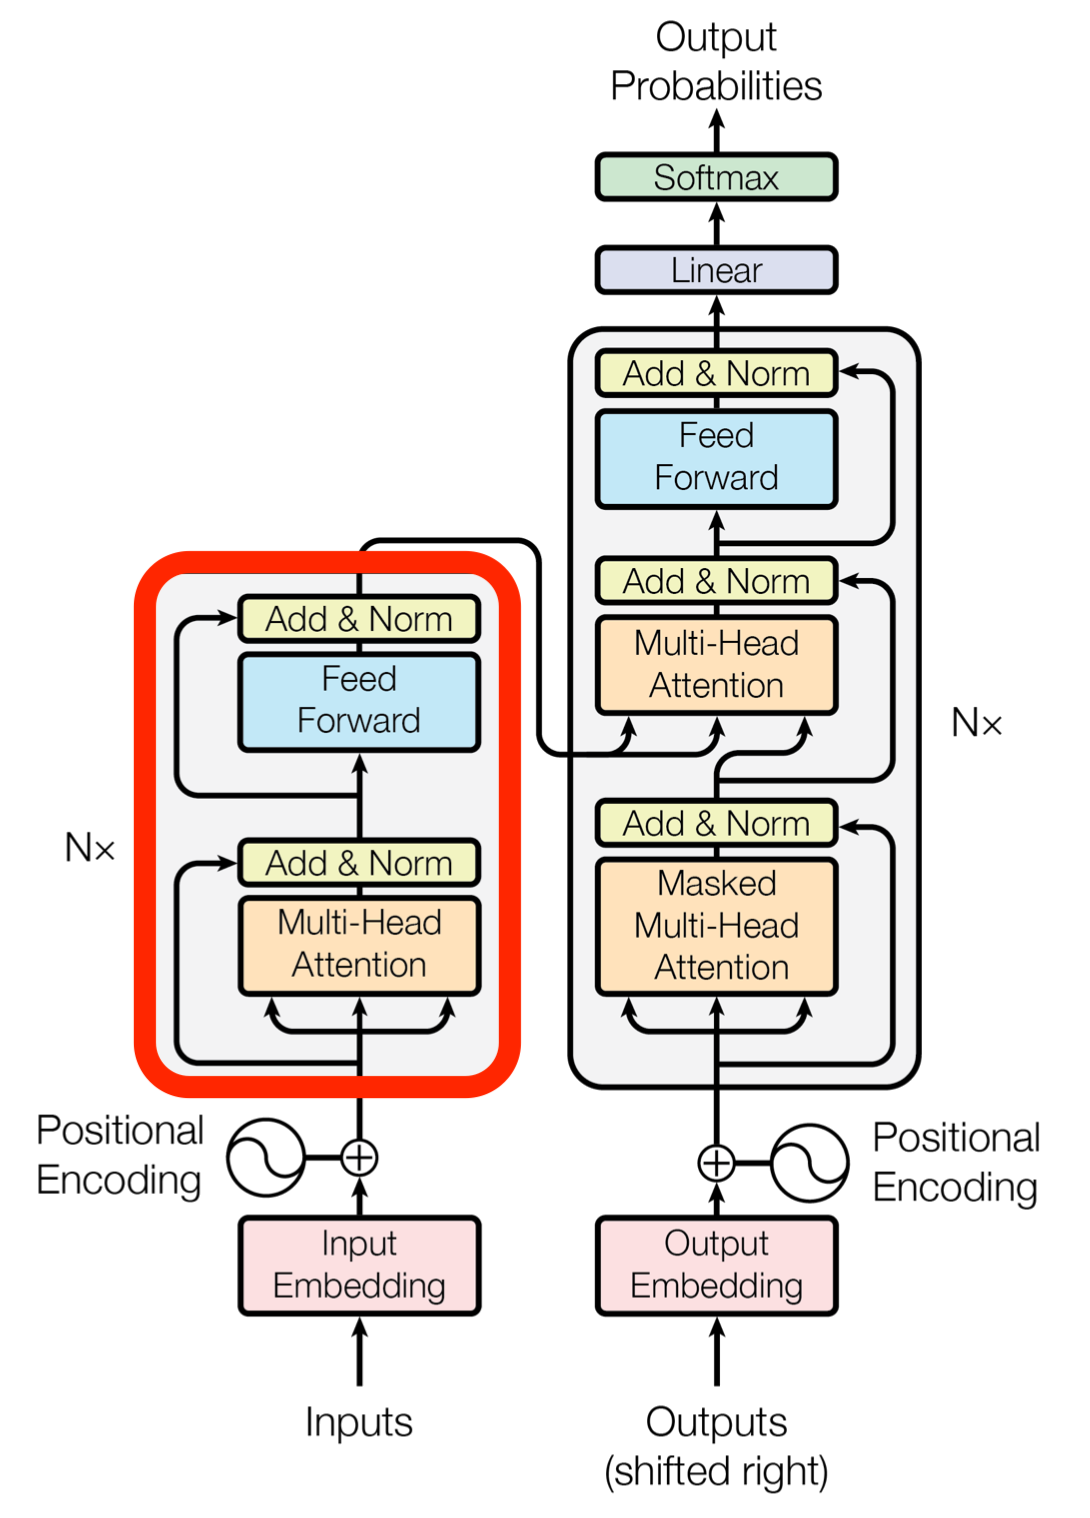
\includegraphics[height=\paperheight]{figures/transformer_encoder_block}
    	\onslide <2> 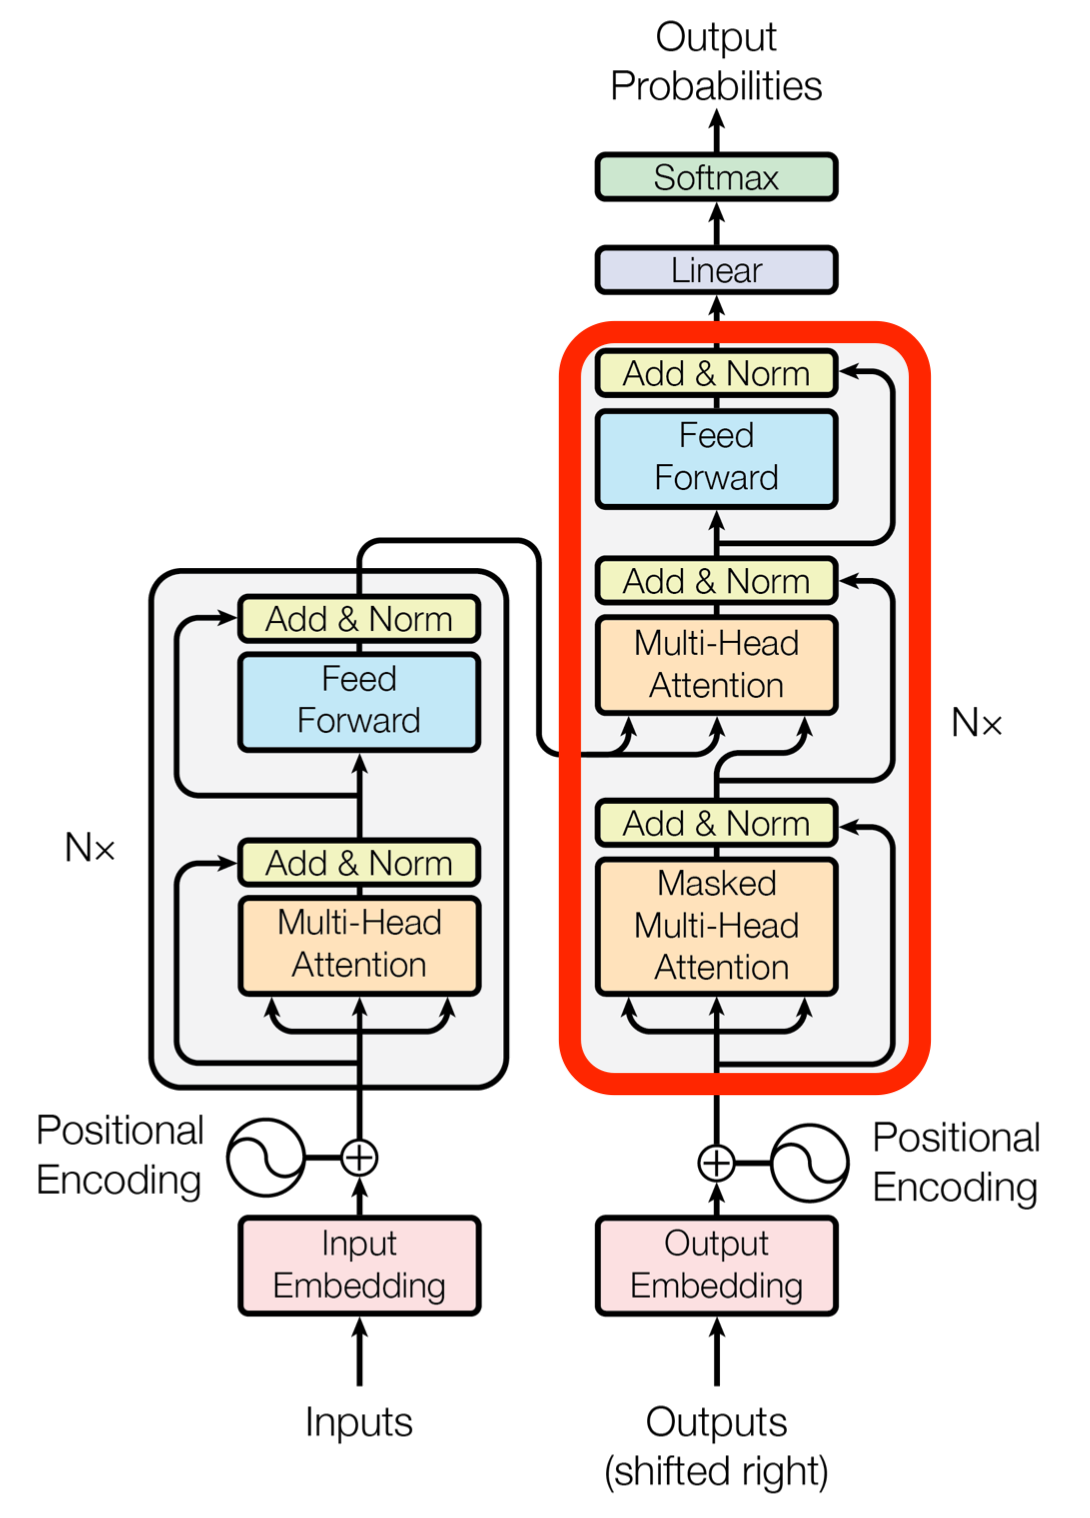
\includegraphics[height=\paperheight]{figures/transformer_decoder_block}
	\onslide <3> 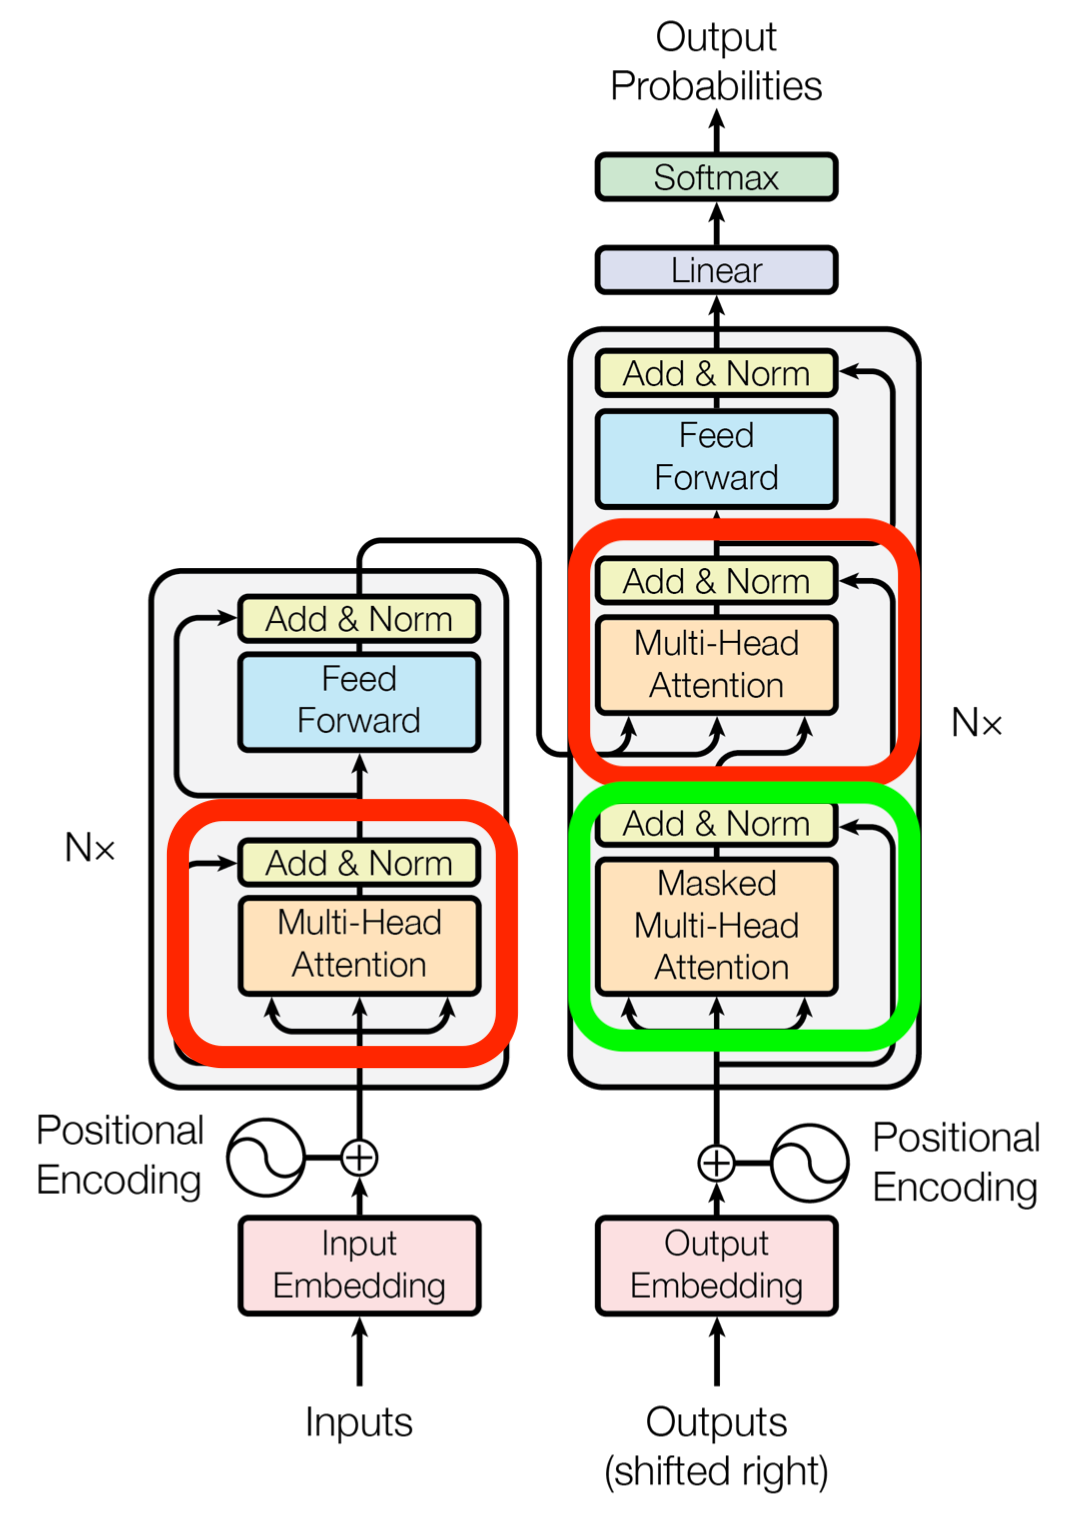
\includegraphics[height=\paperheight]{figures/transformer_multihead_attn}
    \end{overprint}
    \end{figure}
    \end{center}
\end{column}
\end{columns}
\end{frame}

\begin{frame}{The Transformer Architecture}
\centering
Multi-Head Attention
\vspace{.5cm}

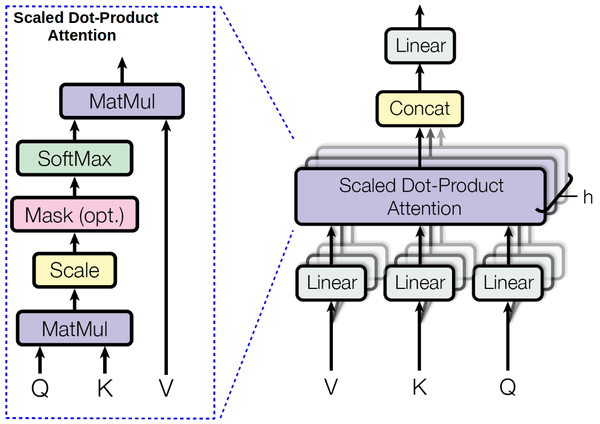
\includegraphics[width=0.45\textwidth]{figures/multihead_attn}

\end{frame}


\begin{frame}{The Transformer Architecture}
\centering
Multi-Head Attention

$$
\mathrm{Attention}(Q, K, V) = \mathrm{softmax}\left( \frac{QK^T}{\sqrt{d_k}} \right)V
$$

$$
\mathrm{head}_i = \mathrm{Attention}\left(QW_i ^Q, KW_i ^K, VW_i ^V\right)
$$

$$
\mathrm{MultiHead}(Q, K, V) = \mathrm{Concat}(\mathrm{head}_1, \mathrm{head}_2, \dots, \mathrm{head}_h)W^O
$$

\begin{itemize}
	\item where $W_i ^Q \in \mathbb{R}^{d_{model} \times d_k}$, $W_i^K \in \mathbb{R}^{d_{model} \times d_k}$, $W_i ^V \in \mathbb{R}^{d_{model} \times d_v}$ and $W_O \in \mathbb{R}^{hd_v \times d_{model}}$, with $d_k = d_v = d_{model} / h$.
	\item \textbf{Dot product attention} is much faster and space efficient than Bahdanau's attention.
	\item The scaling allows the variance of the dot product to be $\approx 1$.
\end{itemize}

\end{frame}

\begin{frame}{The Transformer Architecture}
\centering
Masked Multi-Head Attention
\vspace{.5cm}

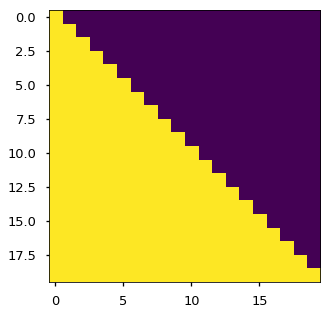
\includegraphics[width=0.4\textwidth]{figures/masked_multihead_attn}

\begin{itemize}
	\item Used so that the model cannot attend to words in the future.
\end{itemize}

\end{frame}

\begin{frame}{The Transformer Architecture}
\begin{columns}
\begin{column}{0.5\textwidth}
\centering
   The Transformer Architecture \cite{vaswani2017attention}

   \vspace{.5cm}
   
   \raggedright
   \begin{itemize}
   	\item No use of recurrent neural networks
	\item We still have the encoder-decoder architecture
	\item Composed of multiple parts :
	\begin{itemize}
		\item Input Embedding
		\item Position Embedding
		\item Multi-Head Attention
		\item Feed Forward Network
	\end{itemize}
   \end{itemize}
\end{column}
\begin{column}{0.5\textwidth}  %%<--- here
    \begin{center}
    \vspace{-1.3cm}
    \begin{figure}
    \begin{overprint}
    	\onslide <1> 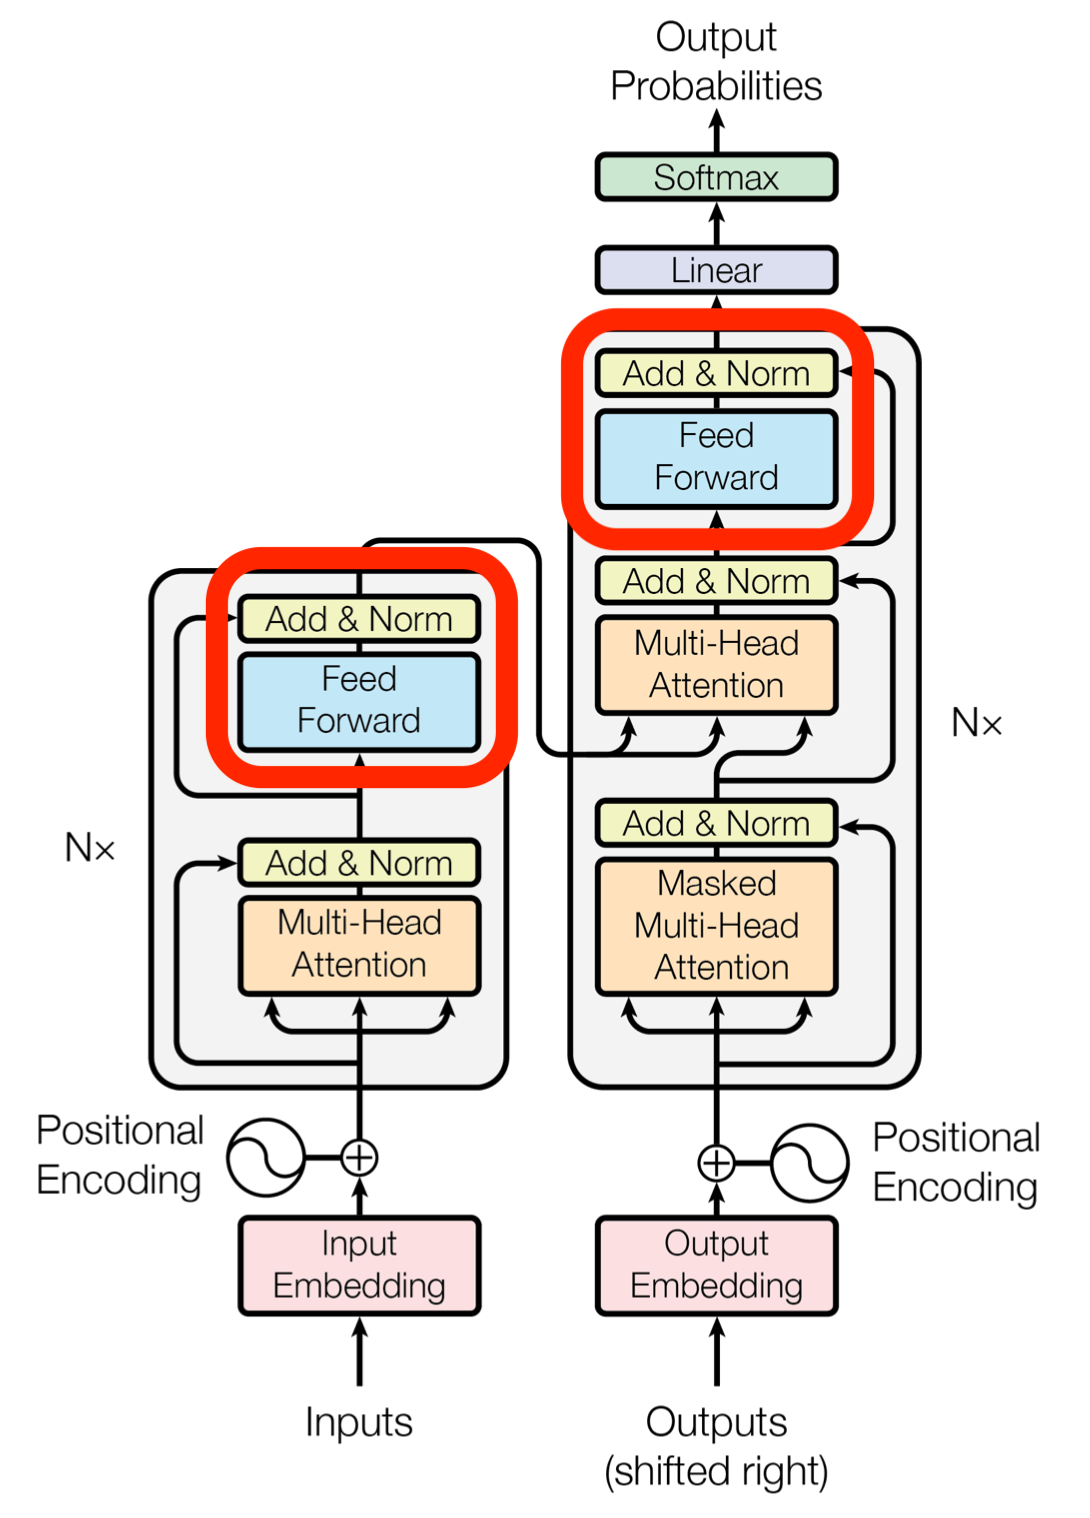
\includegraphics[height=\paperheight]{figures/transformer_feedforward}
    \end{overprint}
    \end{figure}
    \end{center}
\end{column}
\end{columns}
\end{frame}

\begin{frame}{The Transformer Architecture}
\centering
Position-wise feedforward layer
\vspace{.2cm}

$$
\mathrm{FFN}(x) = \mathrm{ReLU}(xW_1 + b_1)W_2 + b_2
$$

\begin{itemize}
	\item where $W_1 \in \mathbb{R}^{d_{model} \times d_{ff}}$ and $W_2 \in \mathbb{R}^{d_{ff} \times d_{model}}$
	\item Can also be seen as two convolutions with kernel of size 1.
\end{itemize}

\end{frame}

\begin{frame}{The Transformer Architecture}

\centering
Residual Connections and Layer Normalization
\vspace{.2cm}

\raggedright

\begin{itemize}
	\item Helps with the gradient propagation for very deep neural networks \cite{he2016deep, ba2016layer}
\end{itemize}
\vspace{.2cm}

\textbf{Residual layer}

$$
\mathrm{Residual}(x) \approx f(x) + x
$$

\textbf{Layer Normalization} 
$$
\mathrm{LayerNorm}(x) \approx \frac{x - \mu}{\sigma + \epsilon}
$$ 

\end{frame}

\begin{frame}{Limitations}
\begin{itemize}
	\item Algorithm is $\mathcal{O}(n^2)$
	\item The maximum size of the input is limited (Solved by Transformer-XL \cite{dai2019transformer})
\end{itemize}
\end{frame}

%%%%%%%%%%%%%%%%%%%%%%%%%%%%%%%%%%%%%%%%%%%%%%%%%%%%%%%%%%%%%%%%%%%%%%%%%%%%%%%%%%%%%%%%
% Transfer Learning in NLP
%%%%%%%%%%%%%%%%%%%%%%%%%%%%%%%%%%%%%%%%%%%%%%%%%%%%%%%%%%%%%%%%%%%%%%%%%%%%%%%%%%%%%%%%
\section{Transfer Learning in NLP}

\begin{frame}{Transfer Learning in NLP}
\centering
\textbf{Two Approaches to Transfer Learning}
\vspace{.3cm}

\begin{columns}
\begin{column}{0.5\textwidth}
   \centering 
   \underline{Feature-based Approach}
   
   \begin{itemize}
   	\item Using pre-trained representations as features for the model
	\item The architecture of the model is task-specific
	\item ex. \textit{Word embeddings, ELMo}
   \end{itemize}
   
\end{column}
\begin{column}{0.5\textwidth}  %%<--- here
    \centering
    \underline{Fine-tuning Approach}
    
    \begin{itemize}
	\item Introduces minimal task-specific parameters
	\item The base model is a pre-trained language model
	\item The final model is trained by fine-tuning the pre-trained model.
	\item ex. \textit{OpenAI-GPT, BERT}
    \end{itemize}

\end{column}
\end{columns}
\end{frame}


%%%%%%%%%%%%%%%%%%%%%%%%%%%%%%%%%%%%%%%%%%%%%%%%%%%%%%%%%%%%%%%%%%%%%%%%%%%%%%%%%%%%%%%%
% Word Embeddings
%%%%%%%%%%%%%%%%%%%%%%%%%%%%%%%%%%%%%%%%%%%%%%%%%%%%%%%%%%%%%%%%%%%%%%%%%%%%%%%%%%%%%%%%
\subsection{Word Embeddings}

\begin{frame}{Word Embeddings}
\centering
\textbf{How to represent words in memory ?}
\vspace{.3cm}

\raggedright
Trivial way is by using a \textit{onehot} representation : 

\begin{itemize}
	\item The word is represented by a vector of length $V$
	\item All of the elements of the vector are $0$ except for one element which is $1$.
	\item $V$ : Size of vocabulary
\end{itemize}

\textit{Example} : 

$$
\mathrm{onehot}_V (\mathrm{cat}) = \left[0, 0, \dots, 0, 1, 0, \dots, 0, 0 \right]
$$

\end{frame}

\begin{frame}{Word Embeddings}
\centering
\textbf{How to represent words in memory ?}
\vspace{.3cm}

\raggedright
Limitations with the \textit{onehot} representation : 

\begin{itemize}
	\item Every word vector is extremely sparse.
	\item Every word is independent from each other.
\end{itemize}

$$
\mathrm{onehot}_V (\mathrm{cat}) \perp \mathrm{onehot}_V (\mathrm{dog})
$$

\end{frame}

\begin{frame}{Word Embeddings}

\centering
\textbf{How to represent words in memory ?}
\vspace{.3cm}

\raggedright
Possible solution : \textbf{Word Embeddings}
\vspace{.3cm}

We project the \textit{onehot} representation of the words in a $n$ dimension space. We \textbf{learn} this new representation.
\vspace{.5cm}

2 simple approaches (\textit{Word2Vec} \cite{mikolov2013distributed, mikolov2013efficient}):
\begin{itemize}
	\item \textit{Continuous Bag of Words (CBOW)}
	\item \textit{Skip-Gram}
\end{itemize}

Other popular approach : \textit{GloVe} \cite{pennington2014glove}

\end{frame}

\begin{frame}{Word Embeddings}
\vspace{.2cm}
\textbf{Continuous Bag of Words (CBOW)}
\begin{itemize}
	\item We use the context to predict the word.
\end{itemize}
\centering
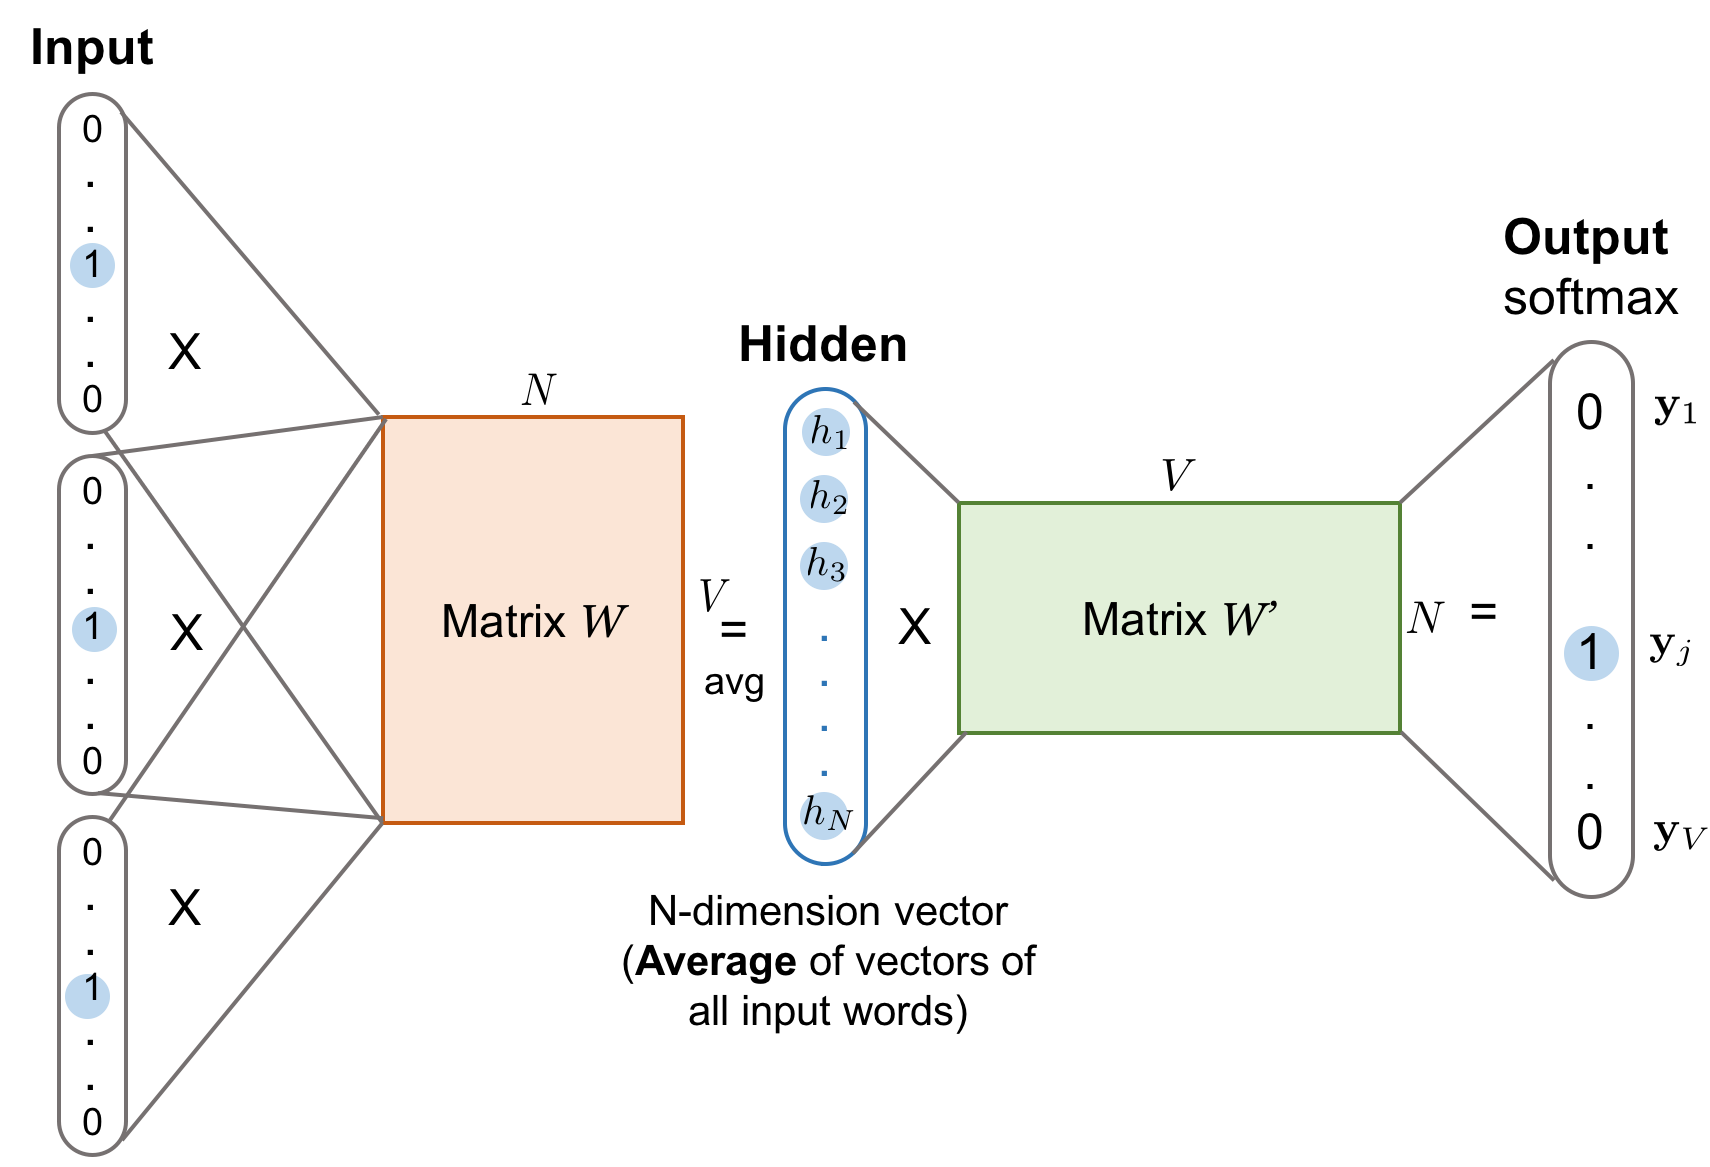
\includegraphics[height=6cm]{figures/word2vec-cbow.png}
\end{frame}

\begin{frame}{Word Embeddings}
\vspace{.2cm}
\textbf{Skip-Gram}
\begin{itemize}
	\item We use the word to predict its context.
\end{itemize}
\centering
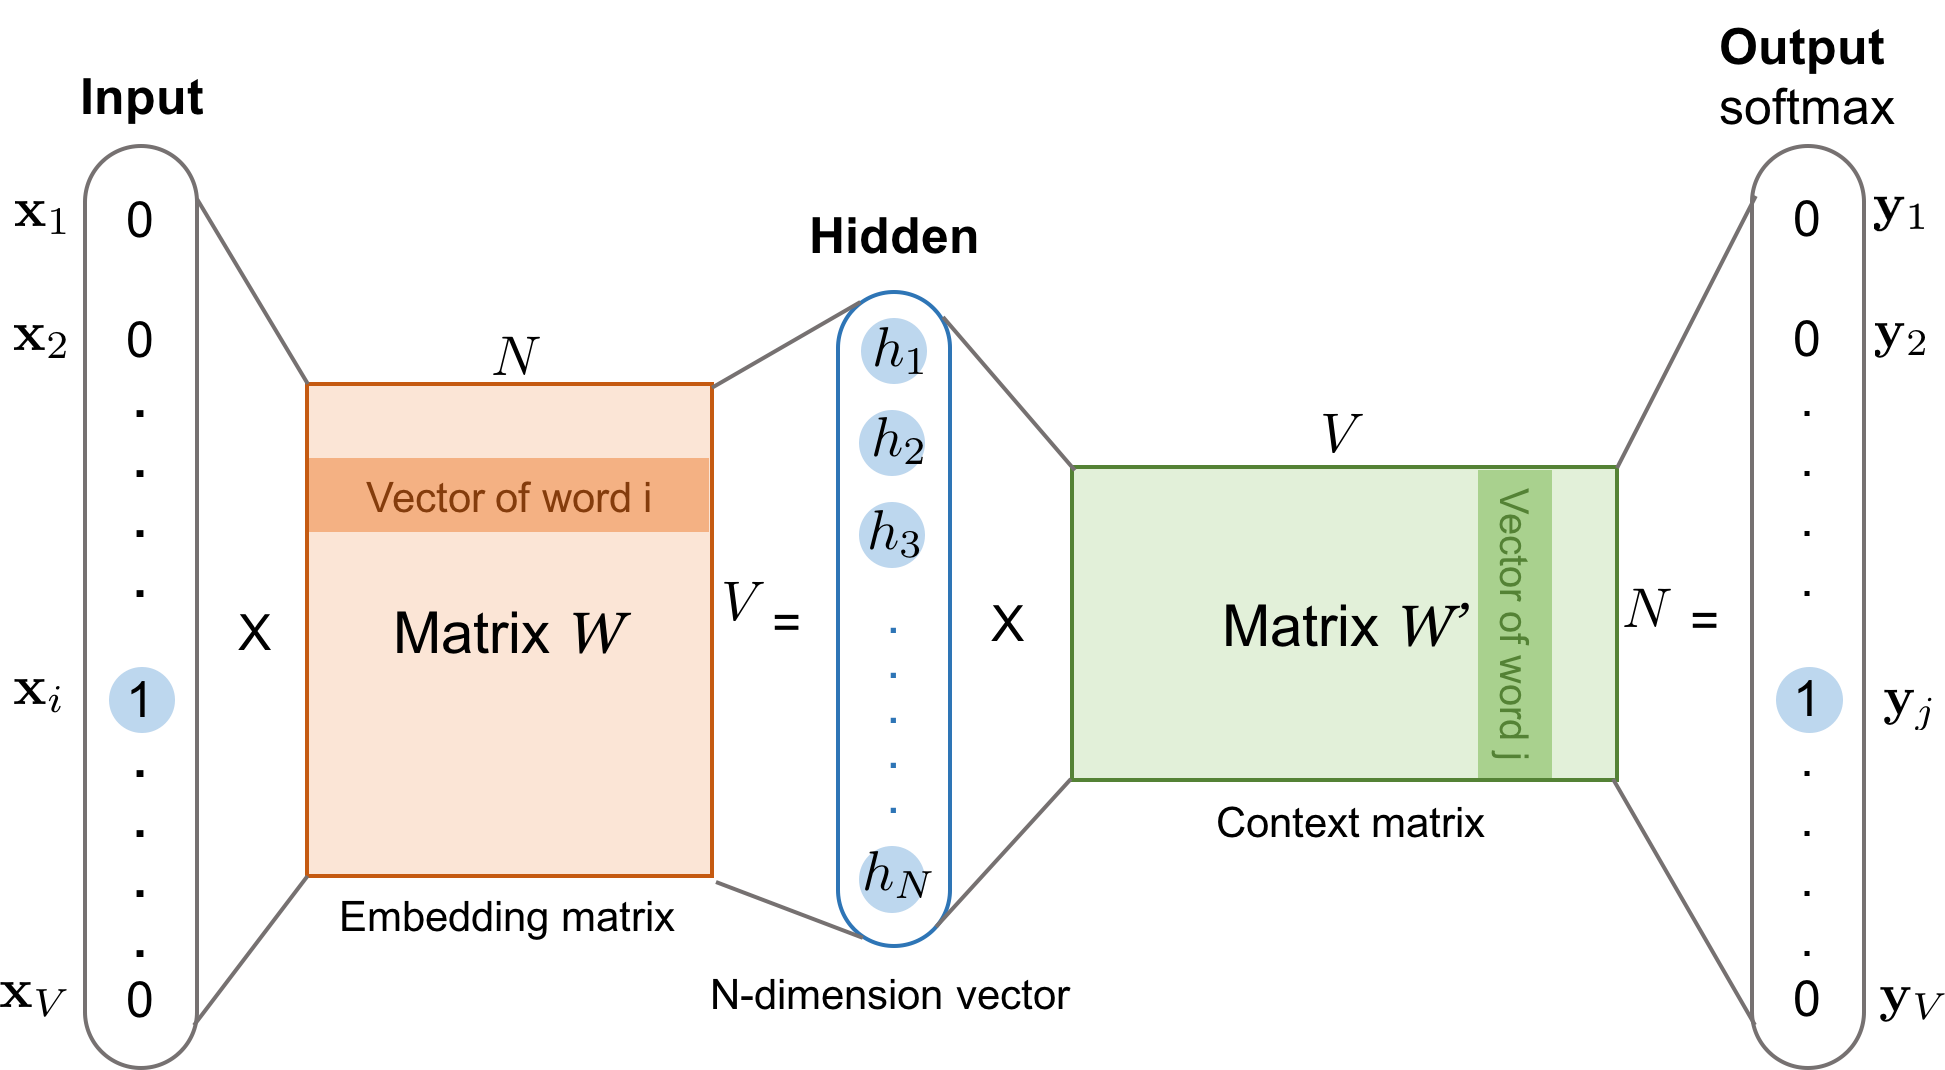
\includegraphics[height=6cm]{figures/word2vec-skip-gram.png}
\end{frame}

\begin{frame}{Word Embeddings}
$$ \mathrm{Repr(man)} - \mathrm{Repr(woman)} + \mathrm{Repr(King)} \approx \mathrm{Repr(Queen)} $$
\centering
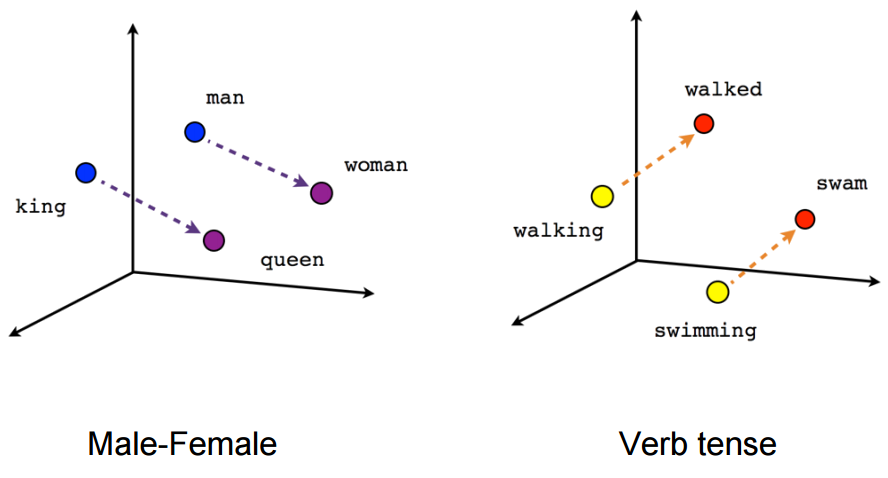
\includegraphics[height=6cm]{figures/male_female_verb_tense.png}

\end{frame}

\begin{frame}{Word Embeddings}
\centering
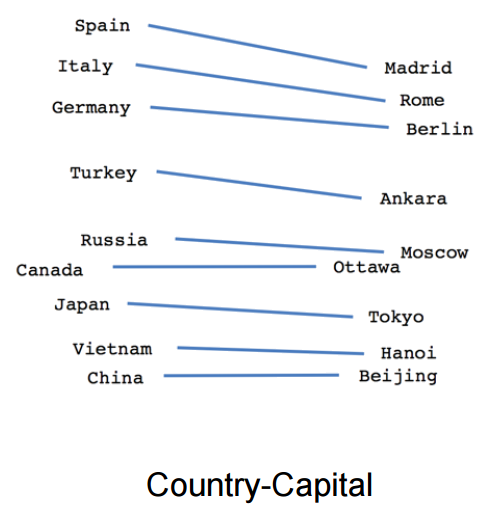
\includegraphics[height=6cm]{figures/capital_country.png}

\end{frame}

\begin{frame}{Word Embeddings}
Limitations with \textit{word embeddings}
\vspace{.3cm}

\begin{itemize}
	\item Some words have multiple possible meaning. Ex :
	\begin{itemize}
		\item I \textbf{play} the piano.
		\item I went to a \textbf{play} yesterday.
	\end{itemize}
\end{itemize}
\vspace{.3cm}

Possible solution : \textbf{Contextualized Word Embeddings} (More on that later...)
\end{frame}

%%%%%%%%%%%%%%%%%%%%%%%%%%%%%%%%%%%%%%%%%%%%%%%%%%%%%%%%%%%%%%%%%%%%%%%%%%%%%%%%%%%%%%%%
% Language Models
%%%%%%%%%%%%%%%%%%%%%%%%%%%%%%%%%%%%%%%%%%%%%%%%%%%%%%%%%%%%%%%%%%%%%%%%%%%%%%%%%%%%%%%%
\subsection{Language Models}

\begin{frame}{Language Models}
\centering
\textbf{The Task}
\vspace{.3cm}

\raggedright
We want to predict the next word based on a history of previous words.

$$
p(\mathbf{x}_n | \mathbf{x_1}, \mathbf{x}_2, \dots, \mathbf{x}_{n-1})
$$
\vspace{.3cm}
\centering

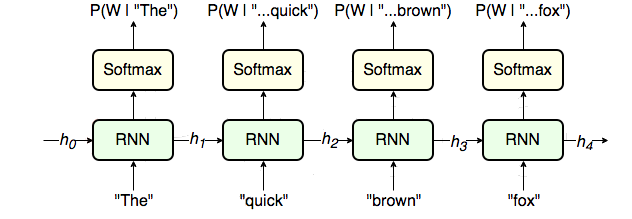
\includegraphics[width=0.8\textwidth]{figures/rnn_language_model}

\end{frame}

\begin{frame}{Language Models}

\begin{description}
	\item [Exemple] Language model imitating \textbf{Shakespeare} \cite{karpathy2015unreasonable}
\end{description}

\begin{quote}
{\small
PANDARUS:\\
Alas, I think he shall be come approached and the day\\
When little srain would be attain'd into being never fed,\\
And who is but a chain and subjects of his death,\\
I should not sleep.\\ \vspace{.5cm}

Second Senator:\\
They are away this miseries, produced upon my soul,\\
Breaking and strongly should be buried, when I perish\\
The earth and thoughts of many states.\\ \vspace{.5cm}

DUKE VINCENTIO:\\
Well, your wit is in the care of side and that. }
\end{quote}

\end{frame}

%%%%%%%%%%%%%%%%%%%%%%%%%%%%%%%%%%%%%%%%%%%%%%%%%%%%%%%%%%%%%%%%%%%%%%%%%%%%%%%%%%%%%%%%
% Contextualized word embeddings
%%%%%%%%%%%%%%%%%%%%%%%%%%%%%%%%%%%%%%%%%%%%%%%%%%%%%%%%%%%%%%%%%%%%%%%%%%%%%%%%%%%%%%%%
\section{Contextualized Word Embeddings}

\begin{frame}{Contextualized Word Embeddings}

\centering
\textbf{ELMo : Embeddings from Language Models \cite{peters2018deep}}
\vspace{.3cm}


\includegraphics[width=0.7\textwidth]{figures/elmo}

\end{frame}

\begin{frame}{Contextualized Word Embeddings}

\centering
\textbf{ELMo : Embeddings from Language Models \cite{peters2018deep}}
\vspace{.3cm}

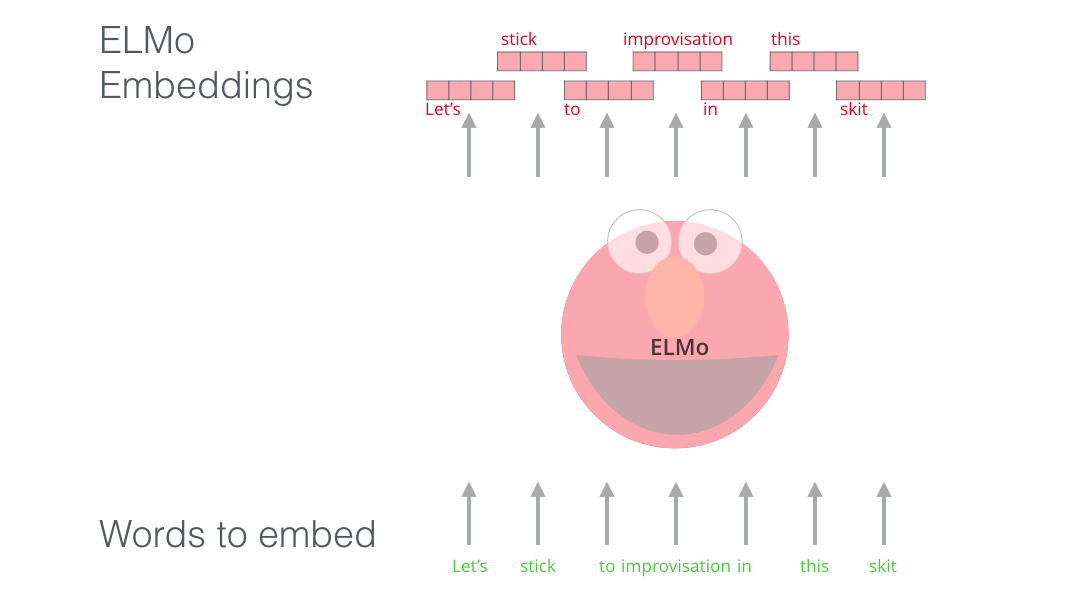
\includegraphics[width=0.7\textwidth]{figures/elmo-word-embedding}

\end{frame}

\begin{frame}{Contextualized Word Embeddings}

\centering
\textbf{ELMo : Embeddings from Language Models \cite{peters2018deep}}
\vspace{.3cm}

\begin{itemize}
	\item Uses Bidirectional LSTM (one language model for each direction)
	\vspace{.2cm}
	\item \textbf{Forward LM} : 
\end{itemize}

$$
p(x_1, \dots, x_n) = \prod_{i=1}^n p(x_i | x_1, \dots, x_{i-1})
$$

\begin{itemize}
	\item \textbf{Backward LM}
\end{itemize}

$$
p(x_1, \dots, x_n) = \prod_{i=1}^n p(x_i | x_{i+1}, \dots, x_n)
$$

\end{frame}

\begin{frame}{Contextualized Word Embeddings}

\centering
\textbf{ELMo : Embeddings from Language Models \cite{peters2018deep}}
\vspace{.3cm}

\begin{itemize}
	\item Instead of just choosing  the output of both direction, we learn a linear combination of the representations at each layer for a given task.
\end{itemize}

$$
R_i = \left\{ h_{i, l} | l = 0, \dots, L \right\}
$$

$$
v_i = f(R_i, \Theta^{\mathrm{task}}) = \gamma^{\mathrm{task}} \sum_{l=0} ^L s_i ^{\mathrm{task}} \mathbf{h}_{i, l} 
$$

\end{frame}

\begin{frame}{Contextualized Word Embeddings}

\centering
\textbf{ELMo : Embeddings from Language Models \cite{peters2018deep}}
\vspace{.3cm}

\begin{itemize}
	\item \textbf{Lower layers} of ELMo are related to \textbf{syntactic tasks} (e.g. POS tagging)
	\item \textbf{Upper layers} of ELMo are related to more \textbf{semantic tasks} (e.g. Word Sense Disambiguation (WSG) where we try to understand the meaning of a given word based on the context)
\end{itemize}

\raggedright
\textbf{Usage}

\begin{itemize}
	\item We use them like we would use normal word embeddings.
\end{itemize}

\textbf{Limitations}

\begin{itemize}
	\item We still need to train a task-specific architecture for the various problems.
\end{itemize}

\end{frame}

\begin{frame}{Transfer Learning in NLP}
\centering
\textbf{Two Approaches to Transfer Learning}
\vspace{.3cm}

\begin{columns}
\begin{column}{0.5\textwidth}
   \centering 
   \underline{Feature-based Approach}
   
   \begin{itemize}
   	\item Using pre-trained representations as features for the model
	\item The architecture of the model is task-specific
	\item ex. \textit{Word embeddings, ELMo}
   \end{itemize}
   
\end{column}
\begin{column}{0.5\textwidth}  %%<--- here
    \centering
    \underline{Fine-tuning Approach}
    
    \begin{itemize}
	\item Introduces minimal task-specific parameters
	\item The base model is a pre-trained language model
	\item The final model is trained by fine-tuning the pre-trained model.
	\item ex. \textit{OpenAI-GPT, BERT}
    \end{itemize}

\end{column}
\end{columns}
\end{frame}

%%%%%%%%%%%%%%%%%%%%%%%%%%%%%%%%%%%%%%%%%%%%%%%%%%%%%%%%%%%%%%%%%%%%%%%%%%%%%%%%%%%%%%%%
% Generative Pre-training (OpenAI-GPT & BERT)
%%%%%%%%%%%%%%%%%%%%%%%%%%%%%%%%%%%%%%%%%%%%%%%%%%%%%%%%%%%%%%%%%%%%%%%%%%%%%%%%%%%%%%%%
\section{Generative Pre-training}

\begin{frame}{Generative Pre-training}
\begin{itemize}
	\item Similar to pretraining a computer vision model on Imagenet and learning other tasks afterwards
	\item Training is done in two steps :
\end{itemize}

\centering

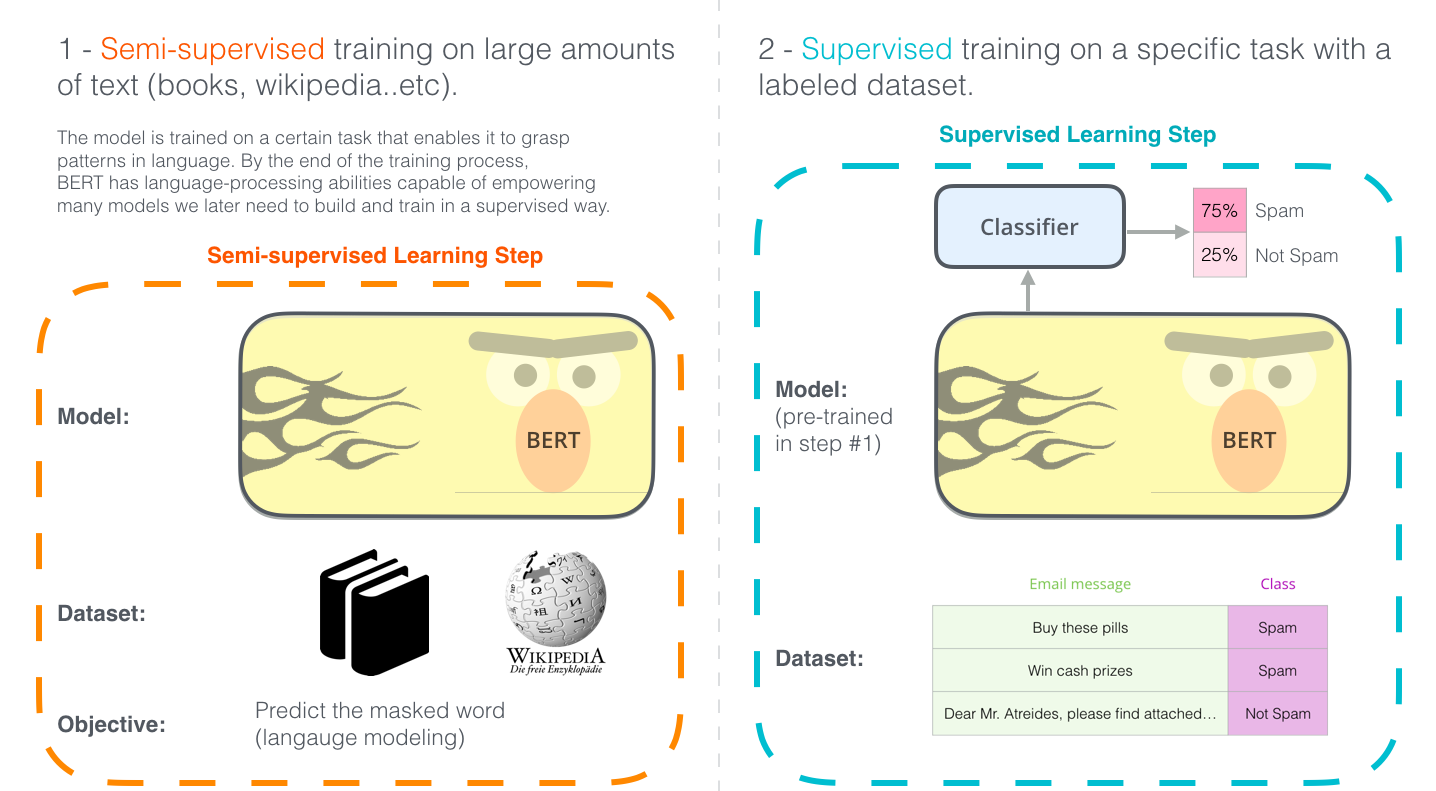
\includegraphics[width=0.7\textwidth]{figures/bert-transfer-learning}

\end{frame}

\begin{frame}{Generative Pre-training}
\centering

\textbf{OpenAI-GPT \cite{radford2018improving}}

\begin{columns}
\begin{column}{0.5\textwidth}
\begin{itemize}
	\item We train a language model using Transformer Decoders.
	\item We fine-tune the model on supervised tasks at the end.
\end{itemize}
   
\end{column}
\begin{column}{0.5\textwidth}  %%<--- here
    \centering

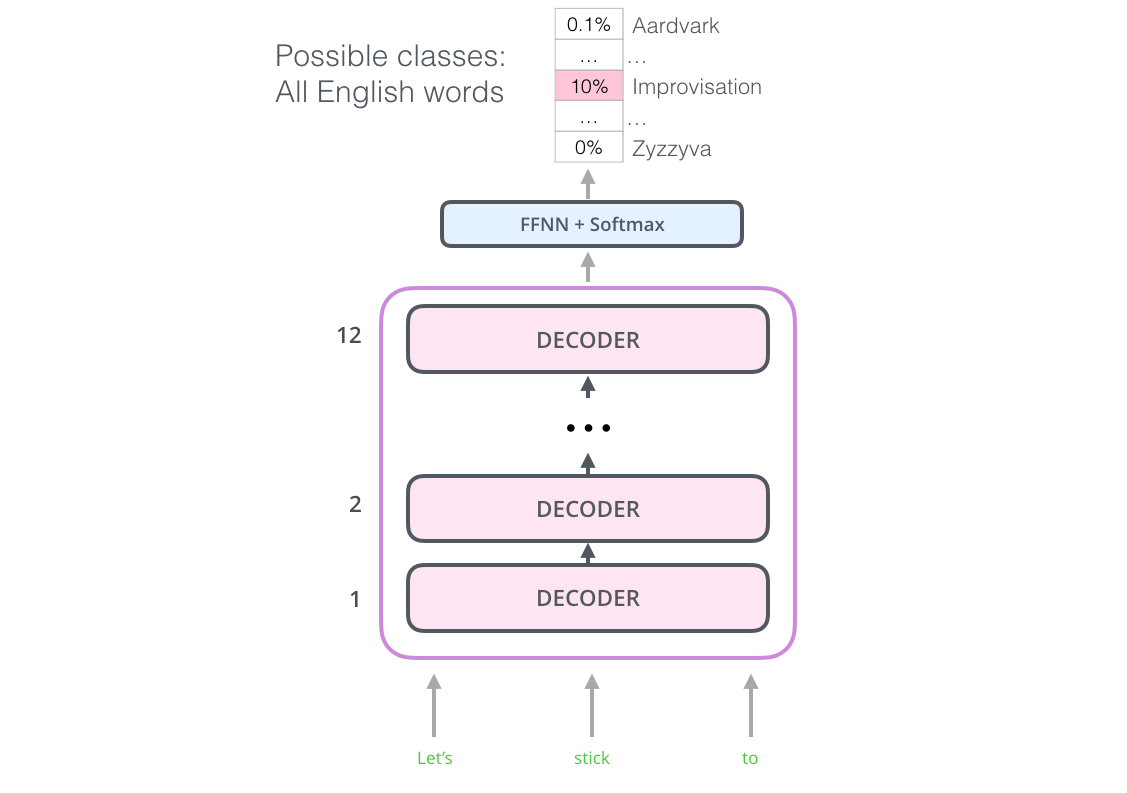
\includegraphics[width=\textwidth]{figures/openai-transformer-language-modeling}

\end{column}
\end{columns}
\end{frame}



\begin{frame}{Generative Pre-training}
\centering
\textbf{OpenAI-GPT \cite{radford2018improving}}

\begin{columns}
\begin{column}{0.5\textwidth}
\begin{itemize}
	\item We train a language model using Transformer Decoders.
	\item We fine-tune the model on supervised tasks at the end.
\end{itemize}
   
\end{column}
\begin{column}{0.5\textwidth}  %%<--- here
    \centering

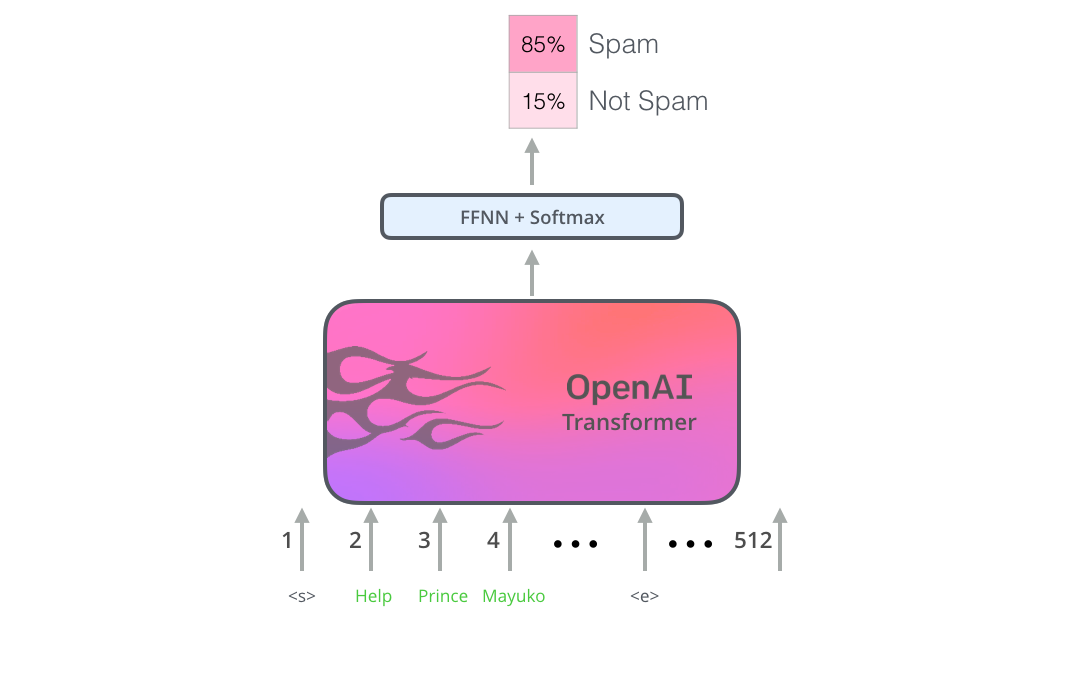
\includegraphics[width=\textwidth]{figures/openai-transformer-sentence-classification}

\end{column}
\end{columns}
\end{frame}

\begin{frame}{Generative Pre-training}
\centering

\textbf{OpenAI-GPT \cite{radford2018improving}}

\begin{columns}
\begin{column}{0.5\textwidth}
\textbf{Limitations}
\begin{itemize}
	\item The language model we have is unidirectional. We want to take into account the full context to predict a word.
\end{itemize}
   
\end{column}
\begin{column}{0.5\textwidth}  %%<--- here
    \centering

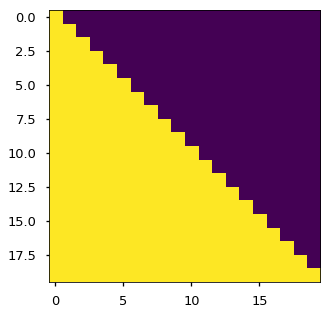
\includegraphics[width=\textwidth]{figures/masked_multihead_attn}

\end{column}
\end{columns}

\end{frame}

\begin{frame}{Generative Pre-training}
\centering
\textbf{BERT : Bidirectional Encoder Representations from Transformers \cite{devlin2018bert}}


\includegraphics[width=0.6\textwidth]{figures/bert}
\end{frame}

\begin{frame}{Generative Pre-training}
\centering
\textbf{BERT : Bidirectional Encoder Representations from Transformers \cite{devlin2018bert}}

\begin{itemize}
	\item We pre-train the model using Transformer Encoders on a \textbf{masked language model problem (MLM)}.
\end{itemize}

$$
p(x_1, \dots, x_n) = \prod_{i=1}^n p(x_i | x_1, \dots, x_{i-1}, x_{i + 1}, \dots, x_n)
$$
\end{frame}

\begin{frame}{Generative Pre-training}
\centering
\textbf{BERT : Bidirectional Encoder Representations from Transformers \cite{devlin2018bert}}

\begin{columns}
\begin{column}{0.3\textwidth}
\begin{itemize}
	\item We pre-train the model using Transformer Encoders on a \textbf{masked language model problem (MLM)}.
\end{itemize}
   
\end{column}
\begin{column}{0.7\textwidth}  %%<--- here
    \centering

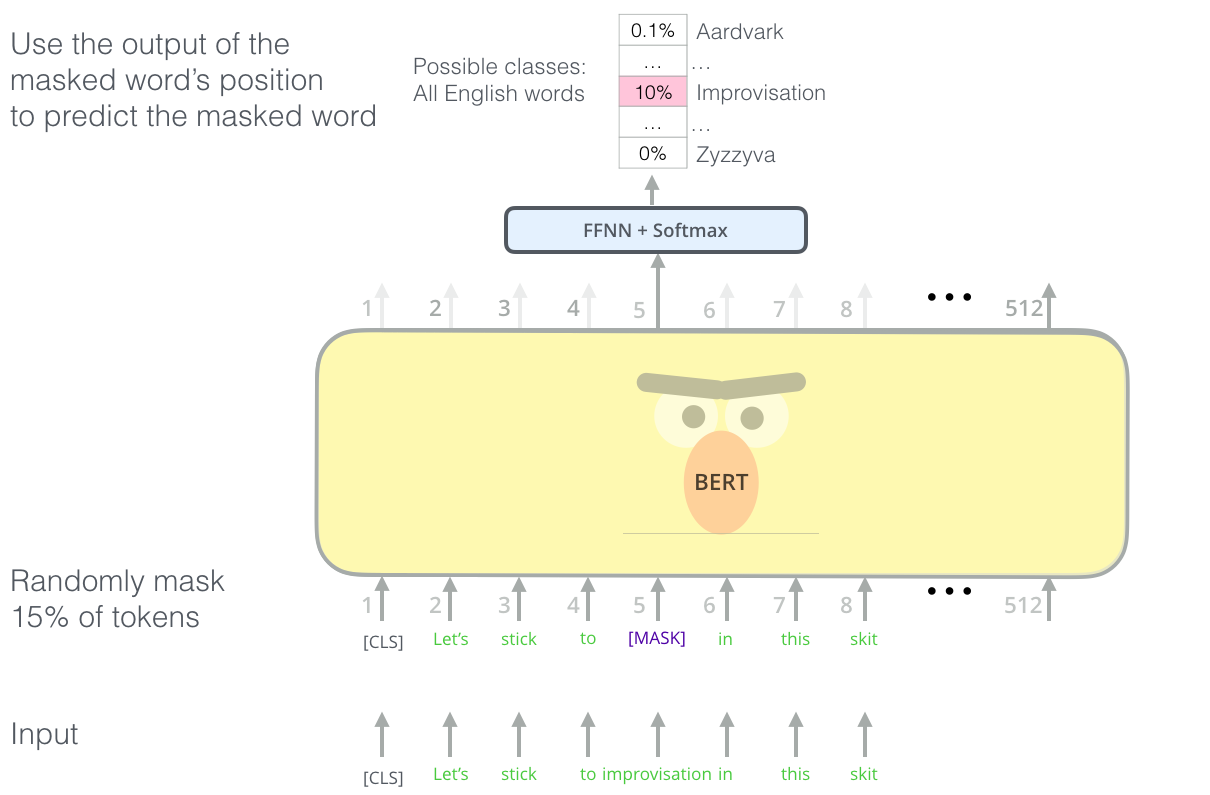
\includegraphics[width=\textwidth]{figures/BERT-language-modeling-masked-lm}

\end{column}
\end{columns}

\end{frame}

\begin{frame}{Generative Pre-training}
\centering
\textbf{BERT : Bidirectional Encoder Representations from Transformers \cite{devlin2018bert}}

\begin{itemize}
	\item Difference between BERT, OpenAI-GPT and ELMo :.
\end{itemize}

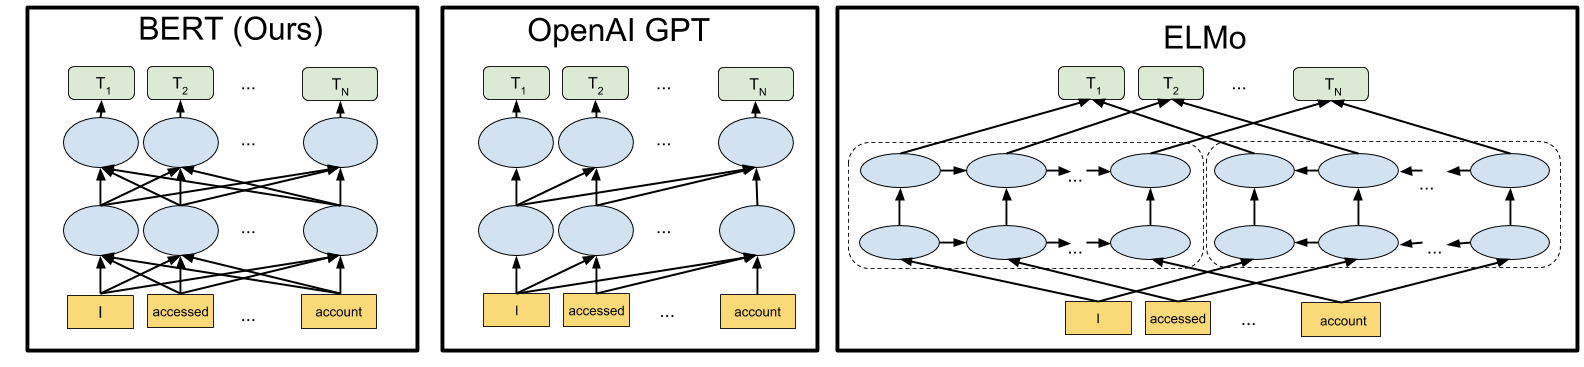
\includegraphics[width=\textwidth]{figures/bert_gpt_elmo_comparison}
\end{frame}

\begin{frame}{Generative Pre-training}
\centering
\textbf{BERT : Bidirectional Encoder Representations from Transformers \cite{devlin2018bert}}

\begin{columns}
\begin{column}{0.3\textwidth}
\begin{itemize}
	\item For tasks taking as input multiple sentences, we want the model to be able to understand the relationship between the various sentences.
	\item To do so, we feed 2 sentences in the model, and ask the model to predict if the second sentence follows the first one.
\end{itemize}
   
\end{column}
\begin{column}{0.7\textwidth}  %%<--- here
    \centering

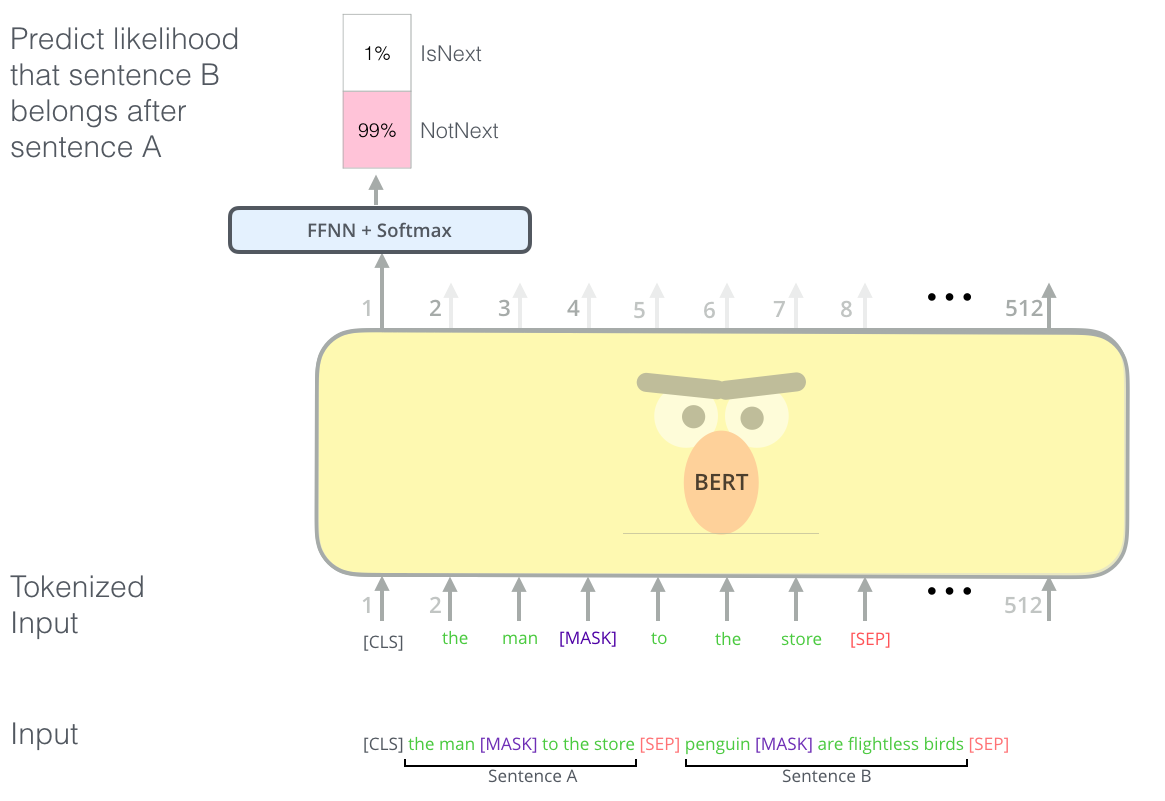
\includegraphics[width=\textwidth]{figures/bert-next-sentence-prediction}

\end{column}
\end{columns}

\end{frame}

\begin{frame}{Generative Pre-training}
\centering
\textbf{BERT : Bidirectional Encoder Representations from Transformers \cite{devlin2018bert}}

\begin{columns}
\begin{column}{0.3\textwidth}
\begin{itemize}
	\item After the pre-training, we can train BERT on downstream tasks easily.
\end{itemize}
   
\end{column}
\begin{column}{0.7\textwidth}  %%<--- here
    \centering

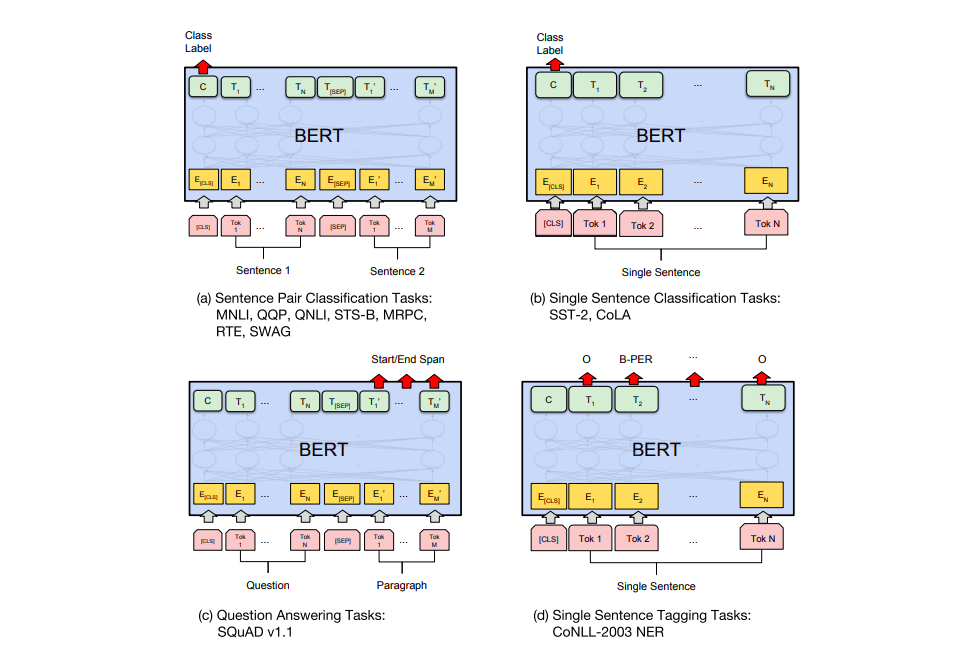
\includegraphics[width=\textwidth]{figures/bert-tasks}

\end{column}
\end{columns}

\end{frame}

\begin{frame}{Generative Pre-training}
\centering
\textbf{BERT : Bidirectional Encoder Representations from Transformers \cite{devlin2018bert}} 

\begin{itemize}
	\item BERT can also be used directly to create contextualized word embeddings just like ELMo !
\end{itemize}

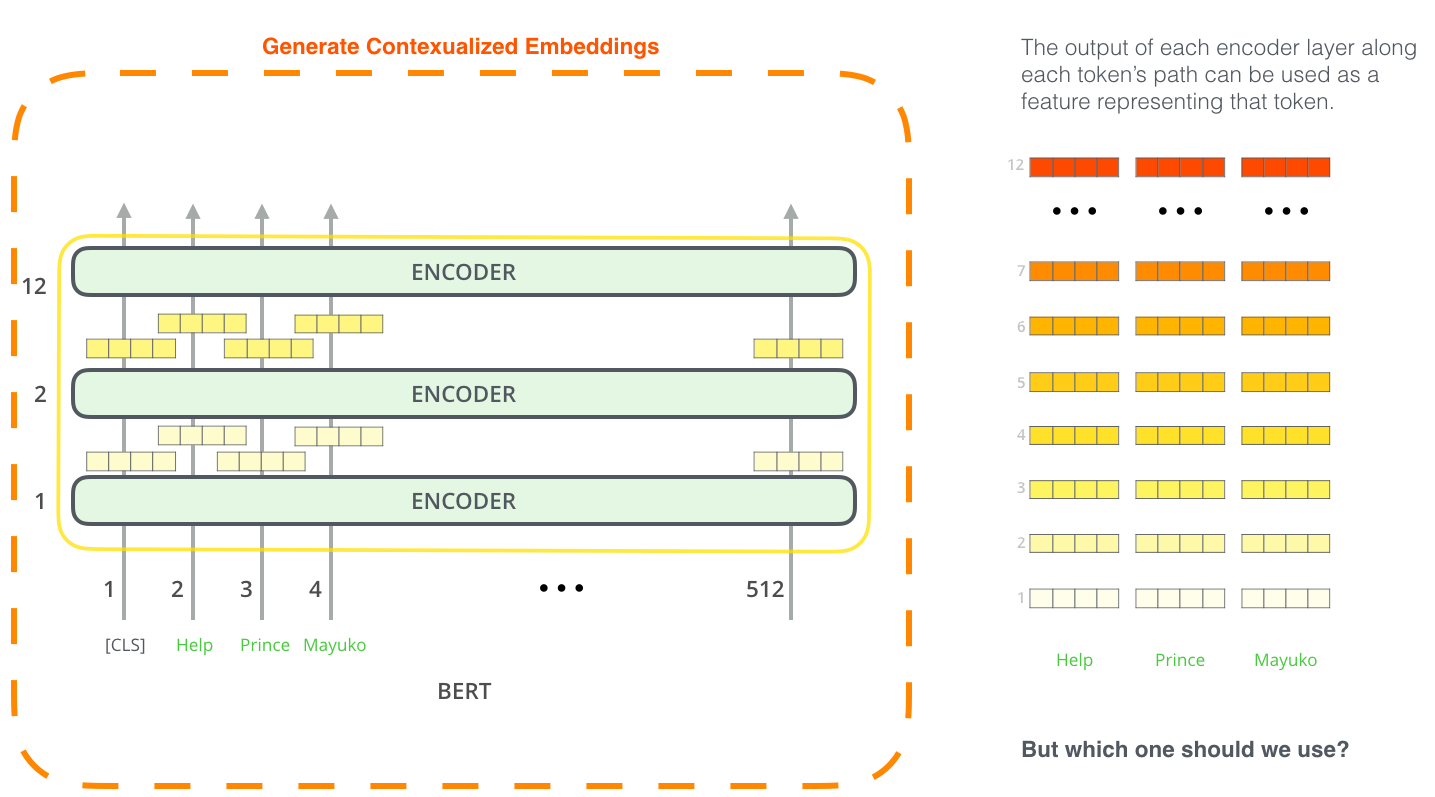
\includegraphics[width=0.7\textwidth]{figures/bert-contextualized-embeddings}
\end{frame}

\begin{frame}{Generative Pre-training}
\centering
\textbf{BERT : Bidirectional Encoder Representations from Transformers \cite{devlin2018bert}}

\begin{itemize}
	\item Which layers should you use?
\end{itemize}

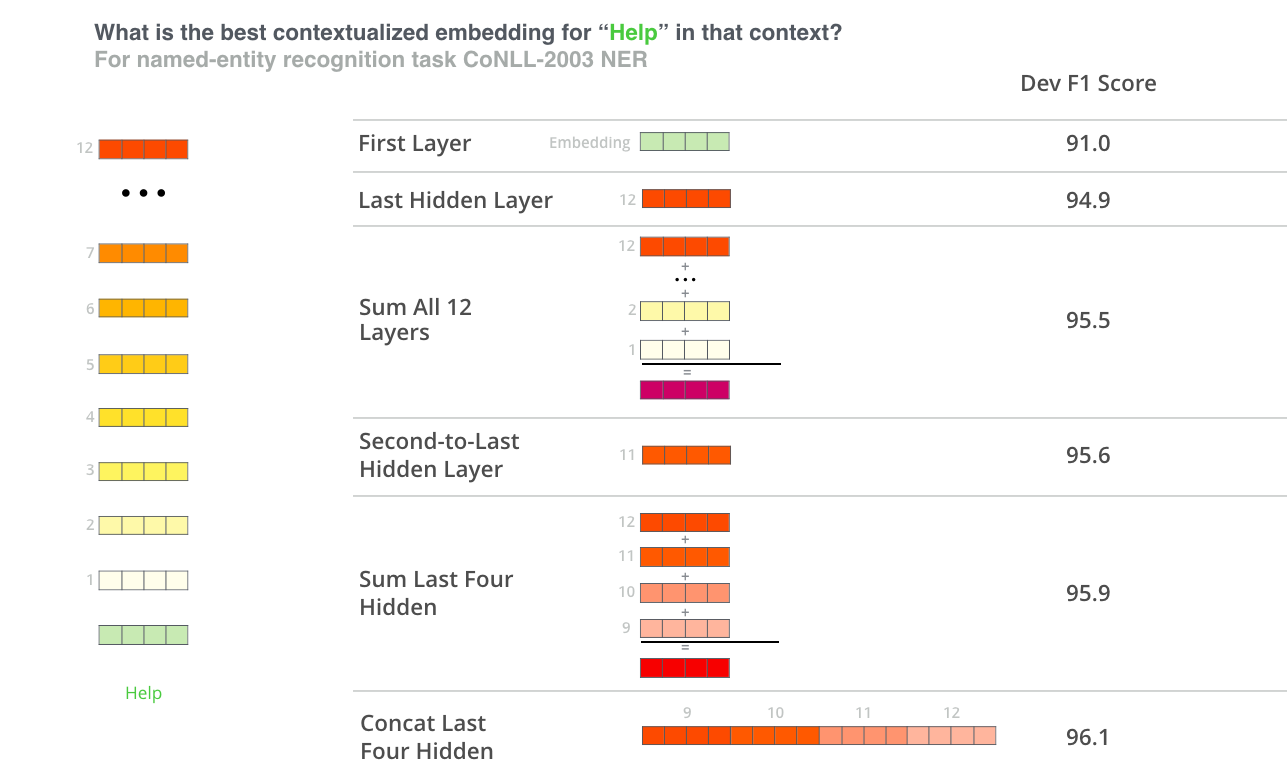
\includegraphics[width=0.7\textwidth]{figures/bert-feature-extraction-contextualized-embeddings}
\end{frame}

\begin{frame}{Generative Pre-training}
\centering
\textbf{BERT : Bidirectional Encoder Representations from Transformers \cite{devlin2018bert}}

\begin{itemize}
	\item BERT is available for anyone to use it (Base and Large version)
	\item Multiple languages are available (English, Chinese, Multi-lingual version trained on Wikipedia)
\end{itemize}

\end{frame}

%%%%%%%%%%%%%%%%%%%%%%%%%%%%%%%%%%%%%%%%%%%%%%%%%%%%%%%%%%%%%%%%%%%%%%%%%%%%%%%%%%%%%%%%
% Implications for the Data Lab
%%%%%%%%%%%%%%%%%%%%%%%%%%%%%%%%%%%%%%%%%%%%%%%%%%%%%%%%%%%%%%%%%%%%%%%%%%%%%%%%%%%%%%%%

\section{Using These Recent Advances in the Data Lab}

\begin{frame}{Using These Recent Advances in the Data Lab}
\begin{itemize}
	\item For the language team, the benefits are evident. Using BERT let's us train supervised models that perform better with less data.
	\item For the UBI team, we could think of training a "driving model" in a similar way that we pretrain BERT. We could then fine-tune this model on various downstream tasks (but which ones?).
\end{itemize}

\centering

\includegraphics[width=0.5\textwidth]{figures/datalab}
\end{frame}

%%%%%%%%%%%%%%%%%%%%%%%%%%%%%%%%%%%%%%%%%%%%%%%%%%%%%%%%%%%%%%%%%%%%%%%%%%%%%%%%%%%%%%%%
% Going Further
%%%%%%%%%%%%%%%%%%%%%%%%%%%%%%%%%%%%%%%%%%%%%%%%%%%%%%%%%%%%%%%%%%%%%%%%%%%%%%%%%%%%%%%%
\section{Going Further}

\begin{frame}{Going Further}

\begin{itemize}
	\item \textbf{\href{http://opennmt.net/}{OpenNMT} : } Open-source implementation of the transformer architecture and multiple other models used in NMT and NLP.
	\item \textbf{\href{http://nlp.seas.harvard.edu/2018/04/03/attention.html}{The Annotated Transformer} : } Step by step explanation of the transformer architecture.
	\item \textbf{\href{http://jalammar.github.io/illustrated-bert/}{The Illustrated BERT, ELMo and co.} :} Step by step explanation of how to use BERT and others.
	\item \textbf{\href{https://lilianweng.github.io/lil-log/2019/01/31/generalized-language-models.html}{Generalized Language Models} :} In-depth explanation of how we went from word embeddings to contextualized word vectors.
	\item \textbf{\href{https://medium.com/huggingface/multi-label-text-classification-using-bert-the-mighty-transformer-69714fa3fb3d}{Multi-label Text Classification using BERT - The Mighty Transformer} :} How to use the pre-trained BERT
\end{itemize}

\end{frame}

%%%%%%%%%%%%%%%%%%%%%%%%%%%%%%%%%%%%%%%%%%%%%%%%%%%%%%%%%%%%%%%%%%%%%%%%%%%%%%%%%%%%%%%%
% References
%%%%%%%%%%%%%%%%%%%%%%%%%%%%%%%%%%%%%%%%%%%%%%%%%%%%%%%%%%%%%%%%%%%%%%%%%%%%%%%%%%%%%%%%

\section*{References}

\begin{frame}[t,allowframebreaks]
\setbeamertemplate{bibliography item}{[\theenumiv]}


  \frametitle{References}
  \nocite*
  \bibliographystyle{siam}
  \bibliography{references}
 \end{frame}

\end{document}